\documentclass[12pt]{beamer}
\usepackage{amsmath}
\usepackage{xcolor}
\usepackage{subfigure}
\usepackage{bbm} 
\usepackage{pgfpages}
\usepackage{tikz}
\usepackage{dcolumn}
\usepackage{booktabs}
\newcolumntype{M}[1]{D{.}{.}{1.#1}}

\usetikzlibrary{positioning,shapes,arrows}

\usepackage{pgf,pgfarrows,pgfnodes,pgfautomata,pgfheaps,pgfshade}
\usetheme{Air}

%\pgfpagesuselayout{4 on 1}[letter,border shrink=5mm]
%\pgfpageslogicalpageoptions{1}{border code=\pgfusepath{stroke}}
%\pgfpageslogicalpageoptions{2}{border code=\pgfusepath{stroke}}
%\pgfpageslogicalpageoptions{3}{border code=\pgfusepath{stroke}}
%\pgfpageslogicalpageoptions{4}{border code=\pgfusepath{stroke}}


\DeclareMathOperator*{\argmax}{arg\,max}

\title[ISMIR 2017 tutorial]{ISMIR 2017 tutorial}


\logo{\pgfputat{\pgfxy(-0.5,7.5)}{\pgfbox[center,base]{\includegraphics[width=1.0cm]{figures/uvic}}}}  
\beamertemplatenavigationsymbolsempty

    \defbeamertemplate{footline}{author and page number}{%
      \usebeamercolor[fg]{page number in head/foot}%
      \usebeamerfont{page number in head/foot}%
      \hspace{1em}\insertshortauthor\hfill%
      \insertpagenumber\,/\,\insertpresentationendpage\kern1em\vskip2pt%
    }
    \setbeamertemplate{footline}[author and page number]{}



\subtitle[Bayes and Markov Listen to Music]{Bayes and Markov Listen to Music} 
\date[2017]{2017}
\author[G. Tzanetakis]{George Tzanetakis}
\institute[University of Victoria]{University of Victoria}
%\logo{\includegraphics[scale=.25]{unilogo.pdf}}

\begin{document}
\frame{\maketitle} % <-- generate frame with title


\AtBeginSection[]
{
\begin{frame}<beamer>[allowframebreaks]{Table of Contents}
\tableofcontents[currentsection,currentsubsection, 
    hideothersubsections, 
    sectionstyle=show/shaded,
]
\end{frame}
}

\section{Motivation} 

\begin{frame}{Motivation} 

Probabilistic modeling is essential in understanding modern techniques
in digital signal processing and machine learning. This course is a
short but comprehensive introduction to probabilistic modeling through
the lens of music information retrieval. 
\end{frame} 


\begin{frame}{Overview} 

  There are 6 units with durations ranging from 15-45 minutes. Each
  unit consists of a set of slides as well as associated hands-on
  demonstrations in the form of Python notebooks.  All the source code
  will be provided to participants and there is considerable
  flexibility in how much time we spend on each unit.

  The units are: 
\begin{itemize} 
\item Motivation - Overview 
\item Discrete Probabilities and Symbolic Music
Processing   
\item Classification using probabilities
\item Dealing with uncertainty and time
\item Probabilistic graphical models
\item Markov Logic Networks 
\end{itemize} 


\end{frame} 



\begin{frame}{Reading resources}

There are many excellent books on probabilistic modeling and machine
learning. Probably my favorite is {\bf ``Machine Learning: a
  Probabilistic Perspective''} by Kevin Murphy. Another good book is
{\bf ``Probabilistic Graphical Models''} by Daphne Koller. A book with
a similar probabilistic perspective that is available online is
{\bf ``Model-Based Machine Learning''} by John Winn and Christopher Bishop
(\url{http://www.mbmlbook.com/}).

  

\end{frame} 

\begin{frame}{Education and Academic Work Experience} 

\begin{itemize} 
\item{1997 BSc in Computer Science (CS), University of Crete, Greece}
\item{1999 MA in CS, Princeton University, USA} 
\item{2002 PhD in CS, Princeton University, USA} 
\item{2003 PostDoc in CS, Carnegie Mellon University, USA}
\item{2004 Assistant Professor in CS, Univ. of Victoria, Canada} 
\item{2010 Associate Professor in CS, Univ. of Victoria, Canada}
\item{2016 Professor in CS, Univ. of VIctoria, Canada}
\item{2010 (renewed 2015) Canada Research Chair (Tier II) in Computer Analysis of AUdio and Music} 
\item{Music theory, saxophone and piano performance, composition,
  improvisation both in conservatory and academic settings}
\end{itemize}
\end{frame} 

\begin{frame}{Research}
Inherently inter-disciplinary and cross-disciplinary work. Connecting
theme: making computers better understand music to create more
effective interactions with musicians and listeners. Audio analysis is challenging due to large volume of data - did big data before it became fashionable. 

\pause  
\begin{columns}
\column{0.5\textwidth}
\begin{itemize} 
\item{Music Information Retrieval} 
\item{Digital Signal Processing} 
\item{Machine Learning} 
\item{Human-Computer Interaction} 
\item{Software Engineering} 
\end{itemize} 

\column{0.5\textwidth}
\begin{itemize}
\item{Artifical Intelligence}
\item{Multimedia}
\item{Robotics} 
\item{Visualization}
\item{Programming Languages} 
\end{itemize} 

\end{columns}
\end{frame}

\section{Introduction}


\begin{frame}{In a nutshell} 
\begin{block}{Quote} 
Essentially, all models are wrong but some are useful. 
\end{block}

\begin{columns}
\column{0.5\textwidth} George Box (1919, 2013). He got interested in
statistics after performing experiments on the effect of poison gas to
small animals in WW II.  \column{0.5 \textwidth}
\includegraphics[scale=0.8]{figures/george_box.jpg}
\end{columns}

\end{frame} 


\begin{frame}{A model-based view of machine learning}

The basic recipe:
\begin{itemize} 
\item {\bf Generate/Sample:} Describe how the data is generated and
  the assumptions you make using a probabilistic model
\item {\bf Learn/Estimate:} Estimate the parameters of the
  probabilistic model using available data (the learning part)
\item {\bf Reason/Infer:} Use the estimated probabilistic model to
  reason about the problem at hand by inference i.e assigning probabilities
  to events of interest that are not known before hand. 
\item {\bf Evaluate:} Examine how well the model performs and what
  types of errors it makes
\end{itemize} 
\end{frame}


\begin{frame}{Important insights}

\begin{itemize}
  \item Understanding notation in addition to the underlying concepts is
  important
\item Separating model from inference
\item Understanding the connection between statistics and probability 
\item Thinking the generative way
\item Probabilistic modeling is all about how to calculate
  probabilities of events that are ``hard'' to estimate from
  probabilities of events that are ``easier'' to estimate
\item Focus on the basic concepts and don't get bogged down in the
  implementation details and the multiple variants
\item Misleading use of language is frequently why probability
  problems can be difficult (for example Monty Hall). In most actual
  applications that's not a problem.
\end{itemize}

\end{frame} 


\section{Discrete Probabilities and Symbolic Music Processing}

\begin{frame}{Overview}

  The main goal of this section is to introduce notation and the very
  basic concepts underlying probabilities. We will start with a very
  simple example and then use the learned concepts to do some simple
  symbolic music modeling using Python.

  \begin{itemize}
  \item{Probability - baysian vs frequentist interpretation}
  \item{Random variables}
  \item{Probabilistic Model}
  \item{Inference}
  \end{itemize} 
\end{frame} 




\begin{frame}{Probability as a framework for quantifying uncertainty} 

  Almost every computational model of some process has to account for
  uncertainty. There are many sources for this uncertainty including:
  measurement noise, wrong model assumptions, lack of knowledge and
  many others. {\it Probability} probably provides the best principled
  framework for quantifying the degree of uncertainty for various
  phenomena in order to build applications and tools that interact
  with the real world.
\end{frame}



\begin{frame}{Frequentist interpretation} 

An event's probability is the limit of its relative frequency in a
large number of trials. This connects to statistics and empirical
experiments.  The initial classical definition of probability was
based on physical idealized symmetry (dice, coins, cards). The
axiomatic formulation of probability by Kolmogorov (1903-1987) in 1933
focuses on operations on probability values rather than the initial
assignment of values.

\end{frame} 

\begin{frame}{Bayesian Probabilities} 

{\bf Probability} summarizes (with a value between 0 and 1) the
uncertainty we have about the world. Probabilities (between 0 and 1)
correspond to intermediate degrees of belief in the truth of a
sentence. Important: the sentence itself is either true or
false. Degree of belief is different than degree of truth and depends 
on our current state of knowledge. 

Consider drawing a card and asking what is the probability it is the
card is the ace of spades. Before looking at the card the probability
is $\frac{1}{52}$ but after it will either be 0 or 1. Therefore, all
probability statements should indicate the evidence used to obtain the
probability estimate. The probability before evidence is obtained is
termed the prior (or unconditional) and after evidence the posterior
(or conditional). 
\end{frame}



\begin{frame}{Frequentists vs Bayesians (xkcd)}
\begin{center} 
 \includegraphics[scale=0.30]{figures/frequentists_vs_bayesians.png}
\end{center} 
\end{frame} 


\begin{frame}{Random variables}

In order to specify the uncertainty about different parts of a problem
that we wish to model we will use {\bf Random Variables}. We specify a
RV with a name and a domain from which it takes values. Discrete
random variables take specific discrete values. For example in music
modeling a random variable for {\it genre} might take the values {\it
  country}, {\it jazz}, and the random variable {\it hasLyrics} might
take the values {\it yes}, {\it no}.
\end{frame} 

\begin{frame}{Assigning probabilities to values of RV} 

  We can associate a probability, a number between $0$ and $1$ to an assignment of a random variable to a value. For example we can have:
  \[
  P(genre = country) = 0.7 
  \]
  
Notice that the sum of the probabilities of all assignments of values
to random variable must add up to 1. This is a normalization
constraint and is essential to being able to combine probability
estimates. Based on it we can state that:
\[
P(genre = jazz) = 0.3 
\]

Notice that I have not said anything about how this number $0.7$ came
about. For now you can think of it as an educated guess. Later we will
talk about how these numbers can be learned from data.
  
\end{frame}



\begin{frame}{Probability Notation} 

{\bf Random Variables} represents a ``part'' of the world whose
``status'' is initially unknown. Each random variable has a domain
that it can take on.  For example, the {\bf RV} $Weather$ can have the
values: $sun$, $rain$, $cloud$, $snow$. Domains can be boolen,
discrete, continuous.
\end{frame}

\begin{frame}{Probability notation continued}

Probabilities are assigned over values in the domain. The notation
${\bf P}(Weather)$ denotes a vector of values for the probabilities of
each individual state of the weather:

\begin{eqnarray*} 
P(Weather = sunny) &= 0.65 \\ 
P(Weather = rain) &= 0.25 \\ 
P(Weather = cloudy) &= 0.07 \\ 
P(Weather = snow) &= 0.03 \\ 
{\bf P}(Weather) &= (0.65, 0.25, 0.07, 0.03) 
\end{eqnarray*}

\end{frame} 

\begin{frame}{Probability} 

Set of all possible outcomes of a random experiment is called the {\bf
  sample space}. $\Omega = {1,2,3,4,5,6}$ is the sample space of
rolling a die. An {\bf event} is a subspace of these outcomes. For
example $E={1,3,5}$ is the event of observing an odd number when
rolling a die. A probability $P$ is a real-valued function defined on
the sample space $\Omega$ that informally assigns values between 0 and 1 to 
all events. 

\end{frame} 

\begin{frame}{Probability properties} 

\begin{itemize} 
\item For any event $E \subset \Omega, \;\;\; 0 \leq P(E) \leq 1$
\item $P(\Omega) = 1$ 
\item For any set of disjoint events, $E_1, E_2, ..., E_k \in \Omega$, 
$P(\cup_{i=1}^{k} E_i) = \sum_{i=1}^{k} P(E_i)$ 
\end{itemize} 
\medskip 
{\bf Note:} These properties help us calculate unknown probabilities
of events based on known probabilities of other events. How the
numbers are assigned to particular events is problem and domain
dependent. They can be assigned based on degrees of belief or they can
be estimated by statistical frequency of occurence.


\end{frame} 


\begin{frame}{Probability distribution and sampling}

  The probabilities associated with every possible value of a random
  variable consitute a {\bf probability distribution}. The process of
  selecting a value randomly according to the probability distribution
  is called {\bf sampling}. It can be viewed as a process of generating
  a sequence of random {\bf samples} and it can help us better understand
  how a particular probabilistic model works. 
\end{frame}

\begin{frame}{Hands-on Example of Probability Distribution \\ and Sampling} 

Jupyter notebook in Python exploring sampling of probability
distributions
  
\end{frame}


\begin{frame}{Incorporating evidence}

  Suppose we introduce another random variable {\it hasLyrics} with two
  values: {\it no} and {\it yes}. We expect that more country
  songs will have lyrics than jazz songs. That means that the
  probability distribution of {\it hasLyrics} depends on whether the
  {\it genre} is {\it country} or {\it jazz}. This is known as a
  conditional probability distribution and is notated as follows:
  \[
  P(hasLyrics = no / genre = jazz) = 0.9 
  \]
  This implies that $P(hasLyrics = yes | genre = jazz) = 0.1$
  \end{frame} 

\begin{frame}{Conditional probability}

  If $genre = country$ then we have:
  \[
  P(hasLyrics  = no | genre=country) = 0.2 
  \]

  We can use the short-hand notation $P(hasLyrics|genre)$ to denote
  the conditional probability distribution that in this case can be
  specified by providing four probabilities (or two using
  normalization). We will call these numbers and in general any
  numbers used to ``specify'' a particular probabilistic model {\bf
    parameters} and use $\theta$ to denote a vector containing them.
\end{frame}

\begin{frame}{Conditional Probability Table}

  We can display all the relevant probabilities using a conditional
  probability table. Notice that the sum of row entries must be equal
  to 1 but NOT the sum of column entries.
  
  \begin{table}
    \begin{tabular}{|c|c|c|}
      \hline 
      genre & hasLyrics = no & hasLyrics = yes \\
      \hline
      country  & 0.2 & 0.8 \\
      \hline 
      jazz & 0.9 & 0.1 \\
      \hline 
      \end{tabular}

    \end{table} 

  \end{frame} 

\begin{frame}{A note about notation}

Frequently when notating a conditional probablity distribution the
short hand $P(hasLyrics|genre)$ is used. Conceptually this expands to
all possible combinations of values of the two random variables
involved. Also some times when the values of random variables in a
problem are unique the name of the random variable is omitted i.e
$P(country)$ instead of $P(genre = country)$. It is important to keep
in mind these conventions as our examples get more complicated.
  
  \end{frame} 



\begin{frame}{Independent variables} 

\begin{definition} 
Two variables $A$ and $B$ are said to be {\bf independent} if $P(A,B) = P(A) P(B)$ (or equivalently $P(A) = P(A|B)$) 
\end{definition} 

Suppose that you toss the same coin twice. If $A$ represent the random
variable of the first toss and $B$ represents the random variable of the
second toss then we can assume that $A$ and $B$ are independent. Evidence
about $B$ will not change our belief about $A$.

Now consider as $A$ the event of rolling a 5 the first time a die is rolled 
and $B$ the event that the sum of numbers of the first roll and the second 
roll is 10. In this case $B$ is not independent of $A$. 

\end{frame} 


\begin{frame}{Our first probabilistic model}

  An illuminating way to think about what we have looked so far is as
  a description of a process that takes into account the various
  sources of uncertainty. First we randomly choose whether the song is
  jazz or country based on the prior distribution (equivalent to
  randomly picking a record from a shelf). There is a $70\%$ chance
  the song will be country and a $30\%$ it will be jazz. Let's suppose
  that it is a country song. Then there is a $20\%$ chance it does not
  have lyrics and and a $80\%$ it has lyrics. Let's consider the event
  that the piece is country and it does not have lyrics. The
  probability of this event is $70\% \times 20\% = 14\%$.
\end{frame}

\begin{frame}{Joint probability} 
  This is the {\bf joint
    probability} of choosing {\it hasLyrics=yes} and {\it genre=jazz}.
  We can use the short hand notation $P(hasLrics, genre)$ to refer to
  this joint probability distribution. Note that the total sum over
  all consituent events of a joint probaiblity should be 1:
  \[
  \sum_{A} \sum_{B} P(A,B) = 1 
  \]
\end{frame}

\begin{frame}{Probabilistic models}
  \begin{definition}{Probabilistic Model}
     \begin{itemize}
     \item   A set of random variables,
       \item A joint probability distribution over these variables
         (i.e. a distribution that assigns a probability to every
         configuration of these variables such that the probabilities
         add up to 1 over all possible configurations).
     \end{itemize}
\end{definition}
\end{frame}

\begin{frame}{Inference}

When we have a probabilistic model we can make predictions, learn
about the values of some random variables given the values of others,
and in general, answer any possibly questions that can be stated about
the random variables. The probablistic model expresses the set of
assumptions we are making about the problem we are tryng to solve and
our uncertainty about them is expressed through probabilities.

Typically we will know the values of some random variables in our
model (evidene) and based on this knowledge we will want to {\bf
  infer} something about the probability distribution of some other
variables.

\end{frame}

\begin{frame}{Product rule}

  We have seen that:
  \[
  P(hasLyrics, genre) = P(genre)P(hasLyrics/genre)
  \]

  This is an example of the {\bf product rule}:
  \[
  P(A, B) = P(A) P(B | A). 
  \]
\end{frame}

\begin{frame}{Sum rule I}
  We can sum the joint probabilities for all possible values of genre
  to ``eliminate'' that variable. 
  \[
  \sum_{hasLyrics} P(hasLyrics, genre = country) = P(genre = country). 
  \]
  More generally using short-hand notation we can express that this
  holds for all values of {\it genre} :
  \[
  \sum_{hasLyrics} P(hasLyrics, genre) = P(genre). 
  \]  
\end{frame}


\begin{frame}{Sum rule II}
More generally the sum rule of probability states: 
  \[
  P(A) = \sum_{B} P(A, B)
  \]


  In this context, the distribution $P(A)$ is known as the marginal
  distribution for $A$ and the act of summing out $B$ is called
  marginalisation.
  
\end{frame}


\begin{frame}{The sum and product rules} 

  The sum and product rules are very general. They apply not just when
  A and B are binary random variables, but also when they are
  multi-state random variables, and even when they are continuous (in
  which case the sums are replaced by integrations). Furthermore, A
  and B could each represent sets of several random variables. For example if $B={C,D}$:
  \[
   P(A, C, D) = P(A) P(C, D | A) 
   \;\;\;\;\;\;\;
    P(A) =\sum_C \sum_D P(A, C, D)
  \]
\end{frame}

\begin{frame}{Inference Example}

    
Recall that the process of obtaining revised probability distributions
after the values of some random variables have been observed, is
called {\bf inference}. Let's look at an example. We know that the
probability of a song is jazz is $30\%$. Suppose that we observe that
the song does not have lyrics. How does this evidence affect the
probability that the song is jazz ? We have:
\[
P(genre = jazz | hasLyrics = no) = \frac{0.3 * 0.9}{0.3 * 0.9 + 0.7 * 0.2} \approx 0.66 
\]
Notice that this {\bf posterior} probability after incorporating evidence is more than twice the original {\bf prior} probability. 
  

\end{frame}

\begin{frame}{Hands-on Example Conditional Probabilities} 

Jupyter notebook in Python exploring conditional probability distributions. 
  
\end{frame}




\section{Classification using Probabilities} 


\begin{frame}{Continuous RVs} 
\begin{block}{Continuous Random Variables}
For continuous variables it is not possible to write out the
distribution as a table as it would have infinite many
values. Instead, the probability that a random variable takes on some
value $x$ is represented as a parameterized function of $x$. For
example we could have $P(X = x) = U[5,20](x)$ express the belief that
the temperature tomorrow will be uniformly distributed between 5 and
20 degrees Celcius. Notice that P(X = 18) should not be interpreted as
the probability that the temperature is exactly 18 degrees which is
zero.  Instead, the temperature in a small region around 18 degrees is
equal to the value in the limit. Sometimes lower case $p(x)$ is used to
differentiate continuous (density) from discrete distributions.
\end{block} 
\end{frame} 



\begin{frame}{Continuous probability functions} 

\begin{table} 
\begin{tabular}{|c|c|c|} 
\hline 
         & Probability Function & Parameters \\ 
\hline 
Gaussian & $p(x) = \frac{1}{\sqrt{2\pi\sigma}}e^{-\frac{1}{2}\frac{(x-\mu)^2}{\sigma^2}}$ & $\mu, \sigma$ \\[10pt] 
\hline 
Binomial & $p(x) = \left ( \frac{n}{x} \right ) p^x(1-p)^{n-x}$ & $n,p$ \\[10pt]
\hline
Poisson  & $p(x) = \frac{1}{x!} \theta^{x} e^{-\theta}$ & $\theta$ \\[10pt] 
\hline 
Exponential & $p(x) = \theta e^{-\theta x}$ & $\theta$ \\[10pt] 
\hline 
\end{tabular} 
\end{table} 


\end{frame}



\begin{frame}{Maximum Likelihood Estimation of Parameters} 
\begin{definition} 
A parametric statistical model is a collection of probability distribution functions each of which is uniquely characterized by a finite dimensional vector of parameters ($\theta$). 
For example Gaussian distributions are characterized by their mean and covariance matrix. 
\end{definition}

\begin{definition}
Given a dataset and set of models find the set of parameters that
maximizes the likelihood of observing the data given the model. In
well-behaved cases this estimation can be performed analytically
rather than numerically using optimization methods. For example the ML
estimate of the mean and covariance matrix are the sample mean and
sample covariance.
\end{definition}
\end{frame}

\begin{frame}{Likelihood} 
\begin{definition} 
The likelihood of a set of data for a particular statistical model assumes that the data is i.i.d (independent and identically distributed). That means that: 
\begin{equation} 
P({\bf x}| M) = \prod_{i}P(x_i | M) = \prod_{i}P(x_i | \theta),
\end{equation} 
\noindent 
where $\theta$ is a vector of parameters characterizing the model $M$
and $x_i$ are the data points. If we consider the equation above as a
function of the $\theta$ for the data point $x_i$ we obtain:
\begin{eqnarray} 
L(\theta | x_1, \dots, x_n) &= \prod_{i}P(x_i | \theta) \\ 
\ln{(\theta | x_1, \dots, x_n)} &= \ln{\prod_{i}P(x_i | \theta)} = \sum_{i} \ln{P(x_i | \theta)}
\end{eqnarray} 
\end{definition}
\end{frame} 



\begin{frame}{Hands-on demonstration of continuous \\ probability
    functions and ML estimation}
\end{frame} 


\begin{frame}{Definition} 
\begin{definition}

Classification (or Supervised Learning) is the machine learning task
of inferring the label (class) of an object (typically represented as
a vector of numbers) by analyzing training data consisting of feature
vectors (representing objects) and associated labels.
\end{definition}
\end{frame} 

\begin{frame}{Example} 
\begin{block}{Example} 

You are given the height, weight of 1000 people as well as a binary
attribute that indicates whether they are professional basketball (or
if you prefer hockey) players or not (\textcolor{red}{training
  set}). You are then given the height and weight of 100 new people
and are asked to predict whether they are professional basketball
players or not (\textcolor{red}{testing set}). The number of correct
predictions is the performance metric.
\end{block}
\end{frame}



\begin{frame}{Train Set and Test Set}

\vspace{-1cm} 
\begin{columns}[t]
\column{0.5\textwidth}
\[
\left( 
\begin{array}{cc|c}
H (cm) & W (kgr) & NBA  \\
190 & \alert<4>{100} & 0 \\ 
\alert<2-3> {195} & \alert<2-4>{110} & \alert<3>{0} \\ 
180 & \alert<4>{85}  & 0 \\ 
\cdots & \\ 
178 & \alert<4>{75}  & 1 \\ 
%165 & \alert<4>{80}  & 1 \\ 
%185 & \alert<4>{90}  & 1 \\ 
\end{array}
\right)
\]


\column{0.5\textwidth}
\[
\left( 
\begin{array}{cc|c}
H(cm) & W(kgr) & NBA \\ 
193 & 102 & ? \\ 
180 & 87  & ? \\ 
200 & 150  & ? \\ 
\cdots & \\ 
168 & 65  & ? \\ 
%175 & 80  & ? \\ 
%187 & 88  & ? \\ 
\end{array}
\right)
\]

\end{columns}

\begin{definition}
A \textcolor{red}{feature matrix} is a 2D matrix \pause where each
row (\alert<2->{instance or sample}) is a feature vector
consististing of numbers (\alert<2->{attribute or feature})
characterizing a particular object \pause and an associated \alert<3->{class
label} (the ground truth). \pause A column corresponds to \alert<4>{attribute} or feature.
\end{definition} 
\end{frame}


\begin{frame}{Classification Formulation} 

\begin{block}{Input}

Training vectors ${\bf x_i} \in R^{d}, i=1,\dots,n$ where $i$ is the
instance index, $n$ is the number of instances, and $d$ is the
dimensionality of the feature vector. Associated ground truth classification labels can be written as integers $y_i$.  
\end{block} 

\end{frame}



\begin{frame}{Classification Operations} 

\begin{block}{Classifier}
A classification algorithm typically supports 2 operations:  
\begin{itemize} 
\item{\bf Train} takes as input a labeled training set (a 2D matrix
  of features and 1D vector of associated labels) and outputs a model
  (a representation of the classifier for that particular problem). 
\pause
\item{\bf Predict} takes as input a trained model and an unlabeled
   testing set (2D feature matrix) and produces a predicted labeled
   test set (1D vector of labels).
\end{itemize} 
\end{block}
\end{frame}

\begin{frame}{Evaluation} 
\begin{block}{Evaluator} 
\begin{itemize}
\item{\bf Evaluate} takes as input a vector of ground truth labels 
and a corresponding vector of predicted labels and calculates various 
classification performance metrics. Classifier is treated as a black box 
\end{itemize}
\end{block} 
\pause 
\begin{example}
{\bf Classification accurancy} can be computed as the percentage of labels that were correctly predicted i.e the ground truth label and the prediction label match. 
\end{example}
\end{frame}

\begin{frame}
\begin{block}{Confusion Matrix} 

This is an $C$ by $C$ matrix $M$ in which each element $M_{i,j}$ shows
the percentage of instances with ground truth class label $i$ that
were predicted as class label $j$. The diagonal element correspond to
the correctly classified instances for each class. The confusion
matrix reveals information about how classification and
misclassification are distributed among different combinations of
classes.
\end{block} 
\end{frame}

\begin{frame}{Example confusion matrix} 
Linear SVM classifier for automatic music genre classificaiton 
($80 \% $) classification accuracy. 

\[
\left( 
\begin{array}{cccccccccc|c}
a  & b	& c & d	& e & f	& g & h	& i & j	& \leftarrow classified \;\;\; as \\ 
79 & 0	& 4  & 4  & 0  & 2 & 6 & 0 & 3 &  2   & a = bl \\ 
0  & 94	& 1  & 0  & 0  & 3 & 0 & 0 & 0 &  2   & b = cl \\ 
5  & 0  & 74 & 1  & 0  & 1 & 3 & 0 & 3 & 13  & c = co \\ 
1  & 0 	& 3  & 74 & 2  & 0 & 1 & 4 & 6 &  9  & d = di \\ 
2  & 0	& 0  & 5  & 78 & 0 & 4 & 3 & 8 &  0  &  e = hi \\ 
2  & 4	& 3  & 0  & 0  & 89 & 1 & 0 & 0	& 1  & f = ja \\ 
3  & 0	& 0  & 5  & 1  & 0  & 83 & 1 & 0 & 7 & g = me \\ 
0  & 0	& 10  &	5 & 4  & 0  &  0 & 72 & 2 & 7	& h = po \\ 
3  & 0	& 5  & 	8 & 11 & 1  &  0 & 2  & 68 & 2	& i = re \\ 
3  & 0	& 17 &	9 & 0  & 0  &  8 & 2 &	6  & 55	& j = ro \\ 
\end{array}
\right)
\]
\end{frame} 




\begin{frame}{Generative Approaches to Classification} 

\begin{block}{Main Idea}

Transform the problem of classification to the multiple
subproblems. Each subproblem consists of estimating the parameters of
a model capable of generating samples similar to the ones associated
with a particular class. In order to transform the problem and perform
the model estimation we first have to review some concepts from
probability and statistics.

\end{block} 
\end{frame}


\begin{frame}{Joint Probability Distribution} 
\begin{block}{Joint Probability Distribution} 
Complete set of RVs used to describe the problem can be represented as
the joint probability distribution. For example the joint distribution 
$P(Weather,Raincoat, Season)$ can be represented as a $2 x 2 x 4$ table. 
\end{block} 
\end{frame}


\begin{frame}{Conditional Probability}
\begin{definition} 
$P(a/b)$ where $a$ and $b$ are propositions.  The probability of $a$
  given that all that we know is $b$. The conditional probability can
  be defined in terms of unconditional probabilities as follows:
\begin{equation} 
P(a/b) = \frac{P(a,b)}{P(b)}
\end{equation}  
\end{definition} 
\end{frame}

\begin{frame}{Conditional Probability Notation}
\begin{block}{Notation} 
\begin{eqnarray}
P(X = x_1, Y = y_1) = P(X = x_1 / Y = y_1) P(Y=y1) \\ 
P(X = x_1, Y = y_2) = P(X = x_1 / Y = y_2) P(Y=y2) \\ 
\dots 
\end{eqnarray}
can be combined with the notation denoting a set of equations: 
\begin{equation} 
{\bf P}(X,Y) = {\bf P}(X/Y) {\bf P}(Y)
\end{equation} 
\end{block} 
\end{frame}

\begin{frame}{Marginal, joint and conditional} 

\begin{table} 
\begin{tabular}{|c|c|c|}
\hline 
             & Male & Female \\  
\hline
Engineering  & 150  &  50    \\ 
\hline 
Humanities   & 20   &  80     \\ 
\hline 
\end{tabular} 
\end{table} 

\begin{align*} 
& P(\mbox{X is Male}) = \frac{150+20}{150+20+50+80} = \frac{170}{300} \approx 0.57  \\
& P(\mbox{X is Female and X in Engineering}) = \\ 
& P(Female, Engineering) = \frac{50}{300} \approx 0.17 \\ 
& P(\mbox{X is Female if we know that X is in Engineering}) = \\ 
& P(Female \ Engineering) = \frac{50}{200} = 0.25 
\end{align*} 


\end{frame} 

%% \begin{frame}{Confidence interval} 
%% Let $\theta$ be the population parameter to be estimated. Then 
%% $(\theta_1, \theta_2)$ is the confidence interval for $\theta$ 
%% at {\bf confidence level} of $1-\alpha$ if 
%% \[
%% P(\theta_1 < \theta < \theta_2) = 1 - \alpha
%% \]
%% \medskip 

%% For a Gaussian distribution with mean of $0$ and variance of $1$ 
%% there is a $95\%$ chance of drawing a number between $-2$ and $+2$. 
%% \end{frame} 



\begin{frame}{Bayes Rule} 
\begin{definition} 
\[
{\bf P}(Y|X) = \frac{{\bf P}(X/Y) {\bf P}(Y)}{{\bf P}(X)} 
\]
\end{definition}
\begin{example}
Suppose $L$ is a rv corresponding to people with lung cancer in a population 
and $S$ is a rv corresponding to the smokers. We have the following data: 
$P(L) = 0.001$, $P(S/L) = 0.9$, $P(S/\hat L)=0.21$. P(L/S) corresponds to the percent of smokers who have lung cancer and can be calculated using the Bayes theorem: 
\[
P(L/S) = \frac{P(S/L)P(L)}{P(S)} = \frac{0.0009}{0.9 * 0.001 + 0.21 * 0.999} = 0.0043 
\]
\end{example}
\end{frame} 

\begin{frame}{What's the big deal ? }

Bayes theorem allows us to ``choose'' in a particular problem the
conditional probabilities that are easier to calculate. For example it
is easier to obtain the probability that someone who has lung cancer
is a smoker than the probability that a smoker has lung cancer.

\hspace{4cm} 
 \includegraphics[scale=0.4]{figures/Thomas_Bayes.png}

\end{frame} 





\begin{frame}{Bayes Classification} 
\begin{equation} 
P(Y/{\bf X}) = \frac{P({\bf X}/Y) P(Y)}{P(\bf X)}
\end{equation}

where $Y$ is the class label and ${\bf X}$ is the feature
vector. Notice that this is a set of equations, one for each class
label in $Y$. Therefore there will be $L$ posterior probabilities one
for each class.  \pause To classify a test instance a {\it Bayesian}
classifier computes these posterior probabilities and selects the
class label corresponding to the maximum posterior. \pause Main
challenge becomes how to estimate $P({\bf X}/Y)$ from the labeled 
training samples. For each class the corresponding training samples
are used to estimate the parameters of the corresponding pdfs.

\end{frame}

\begin{frame}{Bayes Classification} 
 \includegraphics[scale=0.30]{figures/bays_classification.png}
\end{frame} 

\begin{frame}{Bayes Classification - KNN} 
 \includegraphics[scale=0.30]{figures/knn_bayes.png}
\end{frame} 

\begin{frame}{Bayes Classification - GNB GMM} 
 \includegraphics[scale=0.25]{figures/gmm_bayes.png}
\end{frame} 

\begin{frame}{Bayes Error Rate}
\begin{definition} 

Assume that we know the true probability distribution that governs
$P({\bf X}| Y)$. The Bayes error rate is the area in which the class
distributions overlap. For a given feature space, the Bayes Error Rate
is a lower bound on the error rate that can be achieved by any pattern
classifier acting on that space. In general it can only be known
directly if all the class priors and class-conditional likelihoods are
known. The reason is that some of the error is inherent due to
overlapping class densities but some additional error can creep in
because of deficiencies in the classifier and limitations of the
training data.

\end{definition}
\end{frame} 



\begin{frame}{Conditional independence} 
\begin{definition} 
Two variables $A$ and $B$ are said to be {\bf conditionally independent} given 
another variables $C$ if $P(A|C) = P(A|B,C)$. 
\end{definition} 


For example, consider the probability that people are carrying
ubmrellas and that there is heavy traffic. In general those are not
independent as both traffic and umbrella usage will go up if it is
raining. However if we know that it is raining then the probability of
heavy traffic does NOT depend on whether there is increased umbrella
usage (conditional independence).


\end{frame} 

\begin{frame}{Naive Bayes Classifier} 
\begin{definition}
A Naive Bayes classifier estimates the class-conditional probability bu assuming that the attributes are conditionally independent, given the class label $y$. More formally: 
\begin{equation} 
P({\bf X} | Y=y) = \prod_{i=1}^{d} P(X_i | Y=y)
\end{equation}
\end{definition}
\begin{example}
If we know that someone is a professional basketball player then the
probability they have a certain height does not depend on their weight
(this is the naive assumption). However the height of person does
depend on their weight if we don't know whether they are basketball
players or not.

\end{example}
\end{frame}

\begin{frame}{Naive Bayes Classifier} 

The naive assumption about conditional independence of the attributes
allows us to model each attribute separately. For categorical
attributes estimating the conditional probabilities is straightforward
counting based on the training data. For the continuous attributes it
is typically assumed that the probability density function follows a
certain parametric form and the task is to estimate the corresponding
parameters. A common choice is the Gaussian distribution characterized
by two parameters, its mean $\mu$, and variance $\sigma^2$. For each
class $y_i$l, the class-conditional probability for attribute $X_i$
is:

\begin{equation} 
P(X_i = x_i | Y = y_j) =  \frac{1}{\sqrt{2 \pi \sigma_{ij}}} 
\exp^{-\frac{(x_i - \mu_{ij})^2}{2 \sigma_{ij}^2}}
\end{equation} 
\end{frame} 

\begin{frame}{The hoops dataset} 
 \includegraphics[scale=0.5]{figures/hoops_data.png}
\end{frame} 

\begin{frame}{The hoops dataset (Naive Bayes Gaussian)} 
 \includegraphics[scale=0.5]{figures/naive_bayes.png}
\end{frame}

\begin{frame}{Plot Generation}
\begin{block}{Steps for generating plot}  
\begin{itemize}
\item{Plot training set points with colors indicating class labels} 
\pause 
\item{Train classifier} 
\pause
\item{Predict the classes of a dense grid of points (pixels)}
\pause
\item{Color based on the predicted class to visualize decision boundary} 
\pause
\end{itemize}
\end{block}

\end{frame}



\begin{frame}{Characteristics of Naive Bayes Classifiers} 

\begin{itemize}
\item{Robust to isolated noise points especially when there is a lot of data}
\item{Robust to irrelevant attributes as $P(X_i/Y)$ becomes almost uniformly distributed and therefore has little impact to the posterior probability.}
\item{Correlated attributes can degrade the performance} 
\item{Very fast to train and predict} 
\end{itemize}
\end{frame}




\begin{frame}{Hands-on Bernoulli Naive Bayes}

Jupyter notebook for exploring how to estimate the probability
parameters of a simple Bernoulli Naive Bayes classifer for classifying
genre based on lyrics.


\end{frame} 

\section{Clustering} 

\begin{frame}{EM-Algorithm} 

\begin{definition} 
The Expectation Maximization (EM) algorithm is a technique that finds
maximum likelihood estimates in parametric models with incomplete
data. It has many applications in machine learning such as
unsupervised clustering, gaussian mixture modeling, handling missing
values, learning hidden (latent) variables in Bayesian Networks, semi-supervised learning
 and others.
\end{definition} 
\end{frame}

\begin{frame}{EM-algorithm}
\begin{definition} 

The EM-algorithm uses a set of interlocking equations in which the
solution to the parameters requires the values of the latent variables
and vice versa.  It is an iterative (and not guaranteed to be optimal)
procedure that finds the maximum likelihood estimates of the parameter
vector by repeating two steps:
\begin{itemize} 
\item{\bf E-step} Assuming a known model characterized by parameters $\theta$ estimate 
the expected values of the missing data. 
\item{\bf M-step} Treating the estimated values of the missing data as actual values 
re-estimate using ML the parameter vector $\theta$. 
\item{Repeat the {\bf E-step} and {\bf M-step} until there is little change in the 
parameter vector $\theta$. }
\end{itemize} 
\end{definition} 

\end{frame} 

\begin{frame}{Digression - Sufficient Statistics} 

\begin{definition} 
A statistic is a single measure calculated on a set of samples. number 
\end{definition} 


\begin{definition} 
A sufficient statistic for a particular model and associated unknown
parameter is a measure that provide all the information needed for
computing the value of that parameter.
\end{definition} 

\begin{example} 
For a normal distribution $N(\mu, \sigma^2)$ with $\theta = (\mu, \sigma^2)$ the sum of samples and sum of squares $(\sum  x_i, \sum x_i^2)$ are sufficient statistics. 
\end{example} 



\end{frame} 

\begin{frame}{Semi-supervised} 

Basic idea: 

\begin{itemize} 
\item Build model with the labeled samples 
\item Classify unlabeled samples using the model 
\item Retrain model using the newly labeled samples using 
the classifier as ground truth 
\item Repeat the process until the labels don't change signficantly. 
\end{itemize} 

\end{frame}










\begin{frame}{K-means} 

The {\it K-means} algorithms and it's many variants are classic
point-based clustering algorithms that are based on a simple iterative
scheme. Typically the number of desired clusters is provided but there
are techniques for reasonable guesses.

\begin{itemize} 
\item Randomly (or using a simple strategy) pick $K$ initial points to
  be used as cluster centers.
\item Assign each data point to the closest cluster center 
\item Calculate the mean values of the data points belonging to each cluster 
\item Set the cluster centers to be these mean values. 
\item Repeat the previous steps until there is little change in the cluster centers. 
\end{itemize} 


\end{frame} 



\begin{frame}{Gaussian Mixture Model} 

Linear super-position of Gaussians: 
\[
p({\boldsymbol x}) = \sum_{k=1}^{K} p(k)p({\boldsymbol x}/k) 
\] 
\noindent 
where 
\[
\mathcal{N}({\boldsymbol x}| {\boldsymbol \mu}_k, {\boldsymbol \Sigma}_k)
\]
\end{frame} 


\begin{frame}{Sampling from a GMM} 

\begin{itemize} 
\item Generate a uniform random number to determine 
whcih of $K$ components to draw from a sample (based on 
the probabilities $\pi_k$. 
\item Generate a sample from the Gausssian 
$\mathcal{N}({\boldsymbol x}| {\boldsymbol \mu}_k, {\boldsymbol \Sigma}_k)$. 

\end{itemize} 

{\bf Note: } Equivalent procedure generate random samples $N * \pi_k$  
from each component. 

\end{frame} 

\begin{frame}{Fitting the GMM to data} 

Given the data points, we want to estimate: 
\begin{itemize} 
\item The mixing coefficients 
\item The means 
\item The covariances 
\end{itemize} 


If we knew which component generated each data point, we could use ML
solution for each Gaussian separately. The problem is that the data is
unlabelled i.e there is a {\it latent} or hidden variable.

\end{frame} 


\begin{frame}{Labeled vs unlabeled} 

{\bf Note:} K-means gives a good set of initial clusters for the 
EM-algorithm

\end{frame}

\begin{frame}{EM-algorithm} 

If we knew which point contributes to which Gaussian component, the problem 
can be solved more easily but we don't. So the idea is to guess these labels 
and proceed with the estimation. Then using the estimated model, relabel the points, and repeat the process until convergence. 

Latent variable $z_{n,k}$ which is 1 if point $n$ comes from the kth component Gaussian, and otherwise. 

\end{frame}  

\begin{frame}{ML estimation} 

\[
\ln p(\boldsymbol X | \pi, \boldsymbol \mu, \boldsymbol \Sigma) = \sum_{n=1}^{N}  ln \left (  \sum_{k=1}^{K} \pi_k \mathcal{N}(\boldsymbol x_n | \boldsymbol \mu_k \boldsymbol \Sigma_k)  
\right ) 
\]

If oracle gaves us latent variables complete likelihood would be: 
\[
p(\boldsymbol X, \boldsymbol Z | \boldsymbol \mu, \boldsymbol \Sigma, \pi) = 
\prod_{n=1}^{N}\prod_{k=1}^{K} \pi_k^{z_{n,k}} \mathcal{N}(\boldsymbol x_n | \boldsymbol \mu_k, \boldsymbol \Sigma_k) ^{z_{n,k}} 
\]
and log-likehood looks better: 
\[
\ln p(\boldsymbol X, \boldsymbol Z | \boldsymbol \mu, \boldsymbol \Sigma, \pi) =  \sum_{n=1}^{N}\sum_{k=1}^{K} z_{n,k} \left ( \ln \pi_k + ln \mathcal{N}(\boldsymbol x_n | \boldsymbol \mu_k, \boldsymbol \Sigma_k) \right ) 
\]
\end{frame} 


\begin{frame}{EM algorithm} 

\begin{itemize} 
\item Compute $p(Z|X,\theta)$, the posterior distribution over 
$z$ given our current best guess at the values of theta 
\item Compute the expected value of the log likelihood 
$\ln p(X,Z| \theta)$ with respect to the distribution 
$P(Z,X, \theta)$ 
\item Find new $\theta$ that maximizes the function 
\item Iterate 

{\bf Note:} Softening the binary latent variables to continuous ones 
i.e the expected values of the latent variables 

\end{itemize}

\end{frame} 

\begin{frame}{Hands-on example of GMM clustering} 

  Jupyter notebook for showing a variety of GMM covariance types on
  a data set consists of three genres and two audio features
  (mean and standard deviation of spectral centroid) 
  

{\bf Note:} K-means is a special case of Gaussian Mixture Model 
clustering with equal covariance in each component. 

\end{frame} 




\section{Dimensionality Reduction} 

\begin{frame}{Dimensionality Reduction}

The goal of dimensionality reduction techniques is to transform a high
dimensional set of features (or data points) to a space of lower
dimensionality. There are several reasons dimensionality reduction is
desired:
\begin{itemize} 
\item{Some machine learning algorithms have problems handling data of high dimensionality (curse of dimensionality)}
\item{Can lower training (and predicition) time without significantly affecting the classification performance} 
\item{Useful for visualization purposes (2 and 3 dimensions)} 
\end{itemize} 
\end{frame}

\begin{frame}{Principal Component Analysis} 

PCA is used to decompose a multivariate dataset in a set of successive
orthogonal components that explain a maximum amount of the variance at
each stage.  It is an orthogonal linear transform that transforms the
data to a new coordinate system.  It is based on eigen-analysis of the
sample covariance matrix.
\end{frame}

\begin{frame}{Probabilistic Principal Component Analysis} 
  
There is really nice formulation of PCA called {\bf Probabilistic
  Principal Component Analysis} that was proposed in 1999 by
M. Tipping and C. Bishop. The associated paper makes great reading for
seeing how the topics covered in this tutorial such as the
EM-algorithm for ML estimation can be applied to this particular
problem.

\end{frame}

\begin{frame}{PCA geometry} 
\includegraphics[scale=0.35]{figures/pca_geometry.png}
\end{frame} 

\begin{frame}{PCA on Iris dataset}
\includegraphics[scale=0.45]{figures/pca_iris.png}
\end{frame}

\begin{frame}{PCA and LDA} 
\includegraphics[scale=0.45]{figures/pca_lda.png}
\end{frame}

\begin{frame}{Linear Discriminant Analysis} 
\end{frame}

\begin{frame}{Singular Value Decomposition} 
In PCA the principal components are the eigenvectors of the covariance
matrix ${\bf X}{\bf X}^{T}$.  Geometrically in two dimensions the
sample covariance matrix expresses some rotation and scaling of the
data. It is made made diagonal in the transformed space of the
rotated axes. Eigevn values and eigen vectors are possible 
to compute because the covariance matrix is square and symmetric. 

In SVD we directly decompose the data matrix into three matrices: 
\[
{\bf X} = {\bf U}{\bf \Sigma} {\bf V}^T 
\]
In two dimenions it can be viewed as taking any arbitray matrix 
and converting it to an orthogonal matrix (rotation), a diagonal matrix (a stretch) and another orthogonal matrix (a second rotation). 
\end{frame} 

\begin{frame}{Singular-Value Decomposition} 

Similarly to PCA, we can select a subset of the singular values and associated 
vector to create what is called a low rank approximation of the original matrix: 
\[
X: X \approx X_k = U_k \Sigma_k V_k^\top 
\]
After this operation, $U_k \Sigma_k^\top$ is the transformed training
set with $k$ features.  To also transform a test set X, we multiply it
with $V_k: X' = X V_k^\top$
\end{frame} 


\begin{frame}{Relationaship of PCA and SVD} 

It is not necessary to compute the full matrix SVD and then select 
the $k$ singular values components and associated vectors as 
efficient algorithms can only compute the first $k$ singular values. 

This rank reduction is equivalent to PCA on the same data matrix with
the means of every feature removed (centering around zero) - a
standard requirement in PCA. Subtracting the mean feature values when the vectors are sparse can result in them loosing their sparsity therefore SVD is preferred in that case. 
\end{frame} 

\begin{frame}{Latent Semantic Analysis (Indexing)} 

When truncated SVD is applied for text analysis (or indexing) it is
termed latent semantic analysis. Roughly speaking it decomposes the
word count (or tfidf) matrix into a term-concept vector matrix, a
single value diagonal matrix, and a concept-document matrix.

In theory the vectors of the term-concept matrix summarize semantic
information such as words (basketball, nba, Lebron) to hypothesized
concepts (sports) and the vectors of the concept-document matrix
summarize semantic information about which concepts (such as sports,
or news) are contained in each document. To some extent this deals
with the problem of synonyms and polynyms. Typically around 300
dimensions are used in text applications. 

\end{frame} 




\begin{frame}{Probabilistic Latent Semantic Analysis} 

The motivation behind PLSA is similar to LSA but instead of using SVD
to downsize the term-document matrix it is based on a probabilistic
mixture decomposition based on a latent class model.

In this model the probability of a particular word $w$ in a document
$d$ is modeled as a mixture of conditionally independent multinomial
distribution: 

\[
P(w,d) = \sum_c P(c) P(d|c) P(w|c) = P(d) \sum_c P(c|d) P(w|c)
\]

The parameters of the distributions are learned using the EM algorithm. 

\end{frame} 

\begin{frame}{Some terminology: multinomial distribution} 
The multinomial distribution is a generalization of the binomial distribution. 

An exampple: In a recent three-way election for a large country,
candidate A received $20\%$ of the votes, candidate B received $30\%$
of the votes, and candidate $C$ received $50\%$ of the votes. If six
voters are selected randomly, what is the probability that there will
be exactly one supporter for candidate A, two supporters for candidate
B and three supporters for candidate C in the sample?
\end{frame} 


\begin{frame}{Some terminology: Bayesian Estimation} 

Suppose that we want to estimate a parameter $\theta$ on the basis 
of a set of observations ${\bf x}$. Let $L({\bf x}|\theta)$ be the likelihood of observing ${\bf x}$ when the parameter is $\theta$. The maximum likelihood estimate of $\theta$ is: 
\[
\theta_{ML}(x) = \argmax_{\theta} L(x | \theta)
\]

Now assume that a prior distribution $g$ over $\theta$ exists and
instead of a fixed parameter we treat it as a random variable
(Bayesian Statistics). Then the posterior distribution of $\theta$ is as follows: 

\[
f(\theta | x) = \frac{f(x | \theta) \,
  g(\theta)}{\displaystyle\int_{\vartheta \in \Theta} f(x | \vartheta)
  \, g(\vartheta) \, d\vartheta} \!
\]

\end{frame} 

\begin{frame}{MAP estimation} 

The method of maximum a posterior estimation then estimates 
$\theta$ as the mode of the posterior distribution of this random 
variable: 

\[
\hat{\theta}_{\mathrm{MAP}}(x)
= \underset{\theta}{\operatorname{arg\,max}} \ \frac{f(x | \theta) \, g(\theta)}
  {\displaystyle\int_{\vartheta} f(x | \vartheta) \, g(\vartheta) \, d\vartheta}
= \underset{\theta}{\operatorname{arg\,max}} \ f(x | \theta) \, g(\theta).
\]

When the prior distribution $g$ is constant (uniform) then the MAP
estimate coincides with the maximum likelihood estimate. For example
both estimation methods the methods return the sample average as the
estimate of the mean in the case of a Normal Distribution. 

\end{frame} 


\begin{frame}{Latent Dirichlet Analysis} 

{\it Latent Dirichlet Analysis} is a topic modeling technique that is
similar to pLSA. pLSA allows multiple topics in each document but the
possible topic proportions are learned from the document
collection. This means that as a generative model is has trouble
modeling documents with arbitrary topic distributions that were not in
the training collection. LDA introduced by David Blei in 2003 can be
viewed as a Bayesian generalization of pLSA that allows for
classifying new documents and controlling the number of topics.
\end{frame}

\begin{frame}{Generative Model of LDA}
\begin{itemize} 
\item Choose number of words from Poisson distribution 
\item Choose vector of topic proportions according to a Dirichlet 
\item For each word in document 
\begin{itemize} 
\item Choose topic from multinomial distribution over topics 
\item Choose word from multinomial distribution over words conditioned on topic 
\end{itemize} 
\end{itemize} 

\end{frame} 


\begin{frame}{Example of LDA} 
\begin{center}
\includegraphics[scale=0.5]{figures/lda_example.png}
\end{center}
\end{frame} 

\begin{frame}{Inference} 

The LDA model needs to learn various distributions (topics, associated
word probabilities, topic of each word, topic mixture in each
document). This is a problem of Bayesian Inference for which methods
such as variational Bayes or Gibbs sampling can be used.

\end{frame}


\begin{frame}{Hands-on example of PCA, LDA}

  Example of PCA and LDA on 3 genres with high-dimensional audio features.
    
  \end{frame} 



\section{Dealing with uncertainty and time}


\begin{frame}{Markov Chains}

  A {\bf Markov chain} is a sequence of random variables $X1, X2, X3,
  \dots$ with the Markov property, namely that the probability of
  moving to the next state depends only on the present state and not
  on the previous states:

  \[
P(X_{n+1} = x | X_1 = x_1, X_2 = x_2, \dots, X_n = x_n) = P(X_{n+1} =
x | X_{n} = x_n).
\]
  \hspace{4cm} 
 \includegraphics[width=3cm]{figures/markov.png}  
\end{frame}

\begin{frame}{Transition Matrix}
  
The possible values of Xi form a countable set S called the state
space of the chain. A {\bf Markov Chain} can be specified by a
transition matrix with the probabilities of going from a particular
state to another state at every time step.

  \end{frame} 


\begin{frame}{Sequences of observations}

  There are many application areas and music is one of them in which
  we are interesting in modeling probability distributions over
  sequences of observations. We will denote the observation at time
  $t$ by the variable $Y_t$. The variable can be a symbol from a
  discrete alphabet or a continuous variable and we assume that the
  observations are sampled at discrete equally-spaced time intervals
  so $t$ can be an integer-valued time index. 

  Examples in music include the sequence of music intervals that form
  a melody or the sequence of chords in a song. In both of these cases
  the time can be relative to an underlying beat resulting into what is
  called a beat-synchronous representation. 
  

  
\end{frame}


\begin{frame}{Hidden Markov Models (HMMs) graphically} 
\includegraphics[scale=0.3]{figures/hmm.png}
\end{frame}

\begin{frame}{Hidden Markov Models (HMMs) assumptions} 
  Properties:
  \begin{itemize}
    \item The observation at time $t$ is generated by some random
      process whose state $S_t$ is {\it hidden} from the observer.
    \item The hidden states form a Markov Chain i.e given the value
      of $S_{t-1}$, the current state $S_t$ is independent of all
      states prior to $t-1$. The outputs also satisfy a Markov property
      which is that given state $S_t$, the observation $Y_t$ is independent
      of all previous states and observations. 
      \item The hidden state variable $S_t$ is discrete
    \end{itemize} 

\end{frame}

\begin{frame}{The joint distribution of an HMM}
We can write the joint distribution of a sequence of states and observations by using the Markov assumptions to factorize: 
  
  \[
  P(S_{1:T}, Y_{1:T}) = P(S_1) P(Y_1| S_1) \prod_{t=2}^{T} P(S_t|S_{t-1}) P(Y_{t}|S_t)
  \]
\noindent where the notation $X_{1:T}$ indicates the sequence $X_1, X_2, \dots, X_T$. 
\end{frame} 

\begin{frame}{Hidden Markov Models}

  We can view the Hiddean Markov Model graphically as a Bayesian network:
  
  
  \begin{center}
    \includegraphics[scale=0.65]{figures/hmm_bayesian.png}
    \end{center}
\end{frame} 

\begin{frame}{Specifying an HMM}

  So all we need to do to specify an HMM are the following components:
  \begin{itemize}
  \item A probability distribution over the intial state $P(S_1)$
    \item The $K$ by $K$ state transition matrix $P(S_t|S_{t-1})$,
      where $K$ is the number of states
      \item The $K$ by $L$ emission matrix $P(Y_t | S_t)$ if $Y_t$ is
        discrete and has $L$ values, or the parameters $\theta_t$ of
        some form of continuous probability density function if $Y_t$
        is continuous.
    \end{itemize} 
  

  \end{frame} 

\begin{frame}{Motivation for State Space Models}

  Imagine you are tracking a plane on a radar screen that appears as a
  blip that appears every few seconds. You are trying to estimate the
  state (positition and velocity for example) of a physical system
  from noisy observations over time. The problem can be formulated as
  inference in a temporal probability model, where the transition
  model describes the physics of motion and the sensor model describes
  the measurement process.
 
\end{frame}

\begin{frame}{State Space Models}
  In state-space models, a sequence of $D$-dimensional real-valued observation vectors $Y_t$ is modeled by assumign that at each time step $Y_t$ was generated from a $K$-dimensional real-valued hidden state variable $X_t$, and the sequence of X's define a first-order Markov process:
  \[
P(X_{1:T}, Y_{1:T}) = P(X_1) P(Y_1|X_1) \prod_{t=2}^{T} P(X_t|X_{t-1})P(Y_t|X_t)
\]

This factorization is identical to HMMs except that the discrete hidden $S$ state variables are replaced by hidden continuous variables $X$. 

  \end{frame} 

\begin{frame}{Kalman Filter}

  The state transition probability $P(X_t|X_{t-1})$ can be decomposed into
  a deterministic and stochastic components:
  \[
  X_t = f_t(X_{t-1}) + w_t 
  \]
  where $f_t$ is the deterministic transition function, and $w_t$ is zero mean
  random noise vector. Similarly the observation probability $P(Y_t|X_t)$ can
  be decomposed as
  \[
  Y_t = g_t(X_t) + u_t 
  \]
  If these functions are linear and time invariant and the noise variables
  are Gaussian, then the model becomes a linear-Gaussian state-space model
  and it is called a {\bf Kalman Filter} and is used extensively in signal processing. 
\end{frame}

\begin{frame}{Closed Property of HMMs and SSMs}

  What makes HMMs and SSMs special is that their hidden state spaces
  are closed under their respective transition probabilities and
  output models. By that I mean that the hidden state in HMMs is
  assumed to be a multinomial distribution and when the transition
  matrix is applied another multinomial distribution is obtained. In
  SSMs the hidden state is assumed to be Gaussian and after a linear
  transformation and Gaussian noise added it remains a Gaussian hidden
  state. This closed property makes learning and inference
  particularly simple and appealing in these models.

\end{frame}

\begin{frame}{Hands-on example of Markov Chain and HMM} 

  Jupyter notebook for exploring Markov Chains and Hidden Markov
  Models.
\end{frame} 






\section{Bayesian Networks and Inference} 
\begin{frame}{Bayesian Network}

  \begin{definition} 
  A Bayesian network (also known as belief network) is a probabilistic
  graphical model. It represents a set of random variables and their
  conditional dependencies in the form of a directed acyclic graph
  (DAG).
  \end{definition} 

\end{frame}

\begin{frame}{Bayesian Network Example}
\begin{center} 
  \begin{tikzpicture}[
  scale = 0.9, transform shape, 
  node distance=1cm and 0.5cm,
  mynode/.style={draw,ellipse,text width=2cm,align=center}
    ]

\node[mynode] (g) {Genre};
\node[mynode,below=of g] (hl) {HasLyrics};
\path (g) edge[-latex] (hl);

\node[right=0.5cm of g]
{
\begin{tabular}{M{1}M{1}}
\toprule
\multicolumn{2}{c}{Genre} \\
\multicolumn{1}{c}{Jazz} & \multicolumn{1}{c}{Country} \\
\cmidrule{1-2}
0.3 & 0.7 \\
\bottomrule
\end{tabular}
};


\node[left=0.5cm of hl]
{
\begin{tabular}{cM{2}M{2}}
\toprule
& \multicolumn{2}{c}{HasLyrics} \\
HasLyrics & \multicolumn{1}{c}{No} & \multicolumn{1}{c}{Yes} \\
\cmidrule(r){1-1}\cmidrule(l){2-3}
Country & 0.2 & 0.8 \\
Jazz  & 0.9 & 0.1 \\
\bottomrule
\end{tabular}
};



\end{tikzpicture}
\end{center} 
\end{frame} 



\begin{frame}{Extending our BN example}

  This form with multiple features (causes) that are observed being
  conditionally independent of a class (in this case {\bf genre})
  corresponds to a Naive Bayes classifier. It also correspond to
  modeling a medical diagnosis from a set of symptoms.
  
\begin{center} 
  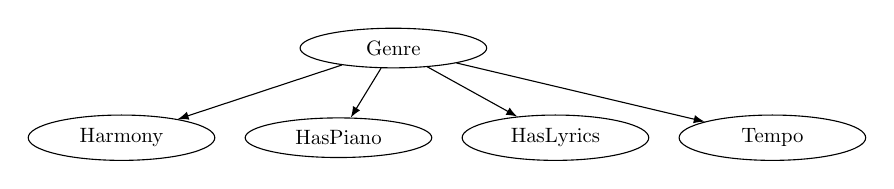
\begin{tikzpicture}[
  scale = 0.75, transform shape, 
  node distance=1cm and 0.5cm,
  mynode/.style={draw,ellipse,text width=2cm,align=center}
    ]

\node[mynode] (hl) {HasLyrics};
\node[mynode,above left=of hl] (g) {Genre};
\node[mynode,left=of hl] (hp) {HasPiano};
\node[mynode,right=of hl] (t) {Tempo};
\node[mynode,left=of hp] (h) {Harmony};
\path (g) edge[-latex] (hl)
(g) edge[-latex] (t)
(g) edge[-latex] (hp)
(g) edge[-latex] (h);
\end{tikzpicture}
\end{center} 
\end{frame}

\begin{frame}{A more complex scenario}

Consider the following scenario. An orchestra manager is trying to
hire musicians. The candidate musicians audition by performing a set
of pieces and are rated by judges. The rating of the judges is based
on the musicianship (weak, strong) and the difficulty of the pieces
they play (low, high). A consensus recommendation letter (weak,
strong) is made stochastically by the judges based solely on their
ratings. In addition, the candidate musicians provide their royal
conservatory of music exam scores which only depend on their
musicianship level. Let's try to express this problem using a Bayesian
network.

  \end{frame} 

\begin{frame}{A more complex BNN}
\begin{center} 
  \begin{tikzpicture}[
  scale = 0.55, transform shape, 
  node distance=1cm and 0.5cm,
  mynode/.style={draw,ellipse,text width=2cm,align=center}
    ]

\node[mynode] (r) {Rating};
\node[mynode,above left=of r] (d) {Difficulty};
\node[mynode,above right=of r] (m) {Musicianship};
\node[mynode,right=of r] (e) {Exam};
\node[mynode,below=of r] (l) {Letter};
\path (d) edge[-latex] (r)
(m) edge[-latex] (r)
(m) edge[-latex] (e)
(r) edge[-latex] (l);


\node[above=of d]
{
\begin{tabular}{M{1}M{1}}
\toprule
\multicolumn{2}{c}{Difficulty} \\
\multicolumn{1}{c}{Low} & \multicolumn{1}{c}{High} \\
\cmidrule{1-2}
0.6 & 0.4 \\
\bottomrule
\end{tabular}
};
\node[above=of m]
{
\begin{tabular}{M{1}M{1}}
\toprule
\multicolumn{2}{c}{Musicianship} \\
\multicolumn{1}{c}{Weak} & \multicolumn{1}{c}{Strong} \\
\cmidrule{1-2}
0.7 & 0.3 \\
\bottomrule
\end{tabular}
};

\node[below right=0.5cm of e, xshift =-1.5cm]
{
\begin{tabular}{cM{2}M{2}}
\toprule
& \multicolumn{2}{c}{Exam} \\
Musicianship & \multicolumn{1}{c}{Low} & \multicolumn{1}{c}{High} \\
\cmidrule(r){1-1}\cmidrule(l){2-3}
Weak & 0.95 & 0.05 \\
High & 0.2 & 0.8 \\
\bottomrule
\end{tabular}
};


\node[left=1.5cm of r, yshift = -1.5cm]
{
\begin{tabular}{ccM{2}M{2}M{2}}
\toprule
& & \multicolumn{3}{c}{Rating} \\
\multicolumn{2}{l}{Difficulty Musicianship} & \multicolumn{1}{c}{*} & \multicolumn{1}{c}{**} & \multicolumn{1}{c}{***} \\
\cmidrule(r){1-2}\cmidrule(l){3-5}
Low  & Weak & 0.3 & 0.4 & 0.3\\
Low  & Strong & 0.05 & 0.25 & 0.7\\
High & Weak & 0.9 & 0.08 & 0.02 \\
High & Strong & 0.5 & 0.3 & 0.2 \\
\bottomrule
\end{tabular}
};

\node[below=of l]
{
\begin{tabular}{ccM{2}M{2}}
\toprule
& & \multicolumn{2}{c}{Letter} \\
\multicolumn{1}{l}{Rating} & \multicolumn{1}{c}{Weak} & \multicolumn{1}{c}{Strong} \\
\cmidrule(r){1-2}\cmidrule(l){3-4}
*   & 0.1  & 0.9  \\
**  & 0.4  & 0.6  \\
*** & 0.99 & 0.01  \\
\bottomrule
\end{tabular}
};



\end{tikzpicture}
\end{center} 

\end{frame}






\begin{frame}{Exact Inference by enumeration}

  Consider how to compute the probability of a particular state for
  example the probability that the candidate has strong musicianship,
  the pieces played are not that difficult, the rating is 2 stars, the
  exam score is high, and the recommendation letter is weak. We can
  use the semantics of Bayesian networks to compute this joint
  probability as follows:
  \begin{eqnarray*}
    & P(m = strong) P(d = low) P(r=**| m = strong, d=low) \\
    & P(e=high | m=strong) P(letter=weak|**)    \\
    &= 0.3 * 0.6 * 0.08 * 0.8 * 0.4 \\
    &= 0.004608
  \end{eqnarray*}

  Any conditional probability distribution can be computed by summing
  terms from the full joint distribution.

\end{frame}

\begin{frame}{Exact Inference}

  This is an example of the chain rule and can be more generally expressed:
  \[
  P(D,M,R,E,L) = P(D)P(M)P(R|M,D)P(E|M)P(L|R)
  \]

  Notice that we can compute the probability of any other event by
  summing over all possible values of the variables we are not
  interested in. For example how would we find P(M,G,E,L) ? How about
  P(M) ? Computing these multiple paths using the product and sum
  rules results in a lot of redundant computations. Variable
  elimination algorithms speed up this exact inference process by
  storing and re-using these common factors.

  
\end{frame}

\begin{frame}{Probabilistic Reasoning}

Consider a particular musician, George and we want to know how likely
he will get a strong recommendation letter. Knowing nothing else this
probability is about $50.2\%$. If we find out that George is not a
strong musician then that probability goes down to around $38.9\%$.

In general we can use our Bayesian Network to answer any combination
of observed, hidden, and query variables. This provides a flexible
formalism that can be used to solve a variety of problems using the
same underlying data and representation. 

\end{frame}

\begin{frame}{Answering a query}
We are looking for the posterior probability distribution of a set of
{\bf query variables}, given values of some observed {\bf evidence
  variables} and we don't care about the values of the remaining {\bf
  hidden variables}.
  
  \[
  P(X,e) = \alpha P(X,e) = \alpha \sum_{y}P(X,e,y)
  \]
  \end{frame} 



\begin{frame}{Factor Graphs}

  Algorithmically and visually it is possible to convert Bayesian Network
  graphs into factor graphs and run {\bf factor graph propagation} making
  more clear the factorization of the joint probability distribution.

  Each black square correpsonds to a CPT and connects the variables
  that are involved in each factor that is multiplied to form
  the joint probability distribution. 

  
\hspace{4cm} 
  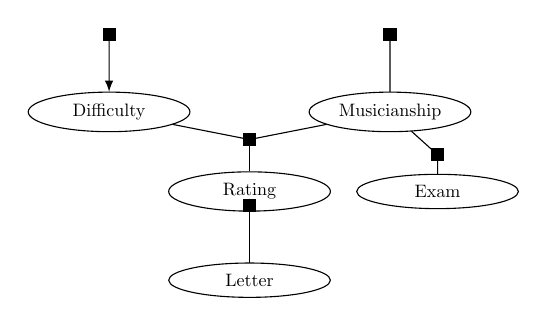
\begin{tikzpicture}[
  scale = 0.65, transform shape, 
  node distance=1cm and 0.5cm,
  mynode/.style={draw,ellipse,text width=2cm,align=center}
    ]

\node[mynode] (r) {Rating};
\node[draw, rectangle,above=of r,fill=black, yshift = -0.5cm] (fr) {};
\node[mynode,above left=of r] (d) {Difficulty};
\node[draw, rectangle,above=of d,fill=black] (fd) {};
\node[mynode,above right=of r] (m) {Musicianship};
\node[draw, rectangle,above=of m,fill=black] (fm) {};
\node[mynode,right=of r] (e) {Exam};
\node[draw, rectangle,above=of e,fill=black, yshift = -0.75cm] (fe) {};
\node[mynode,below=of r] (l) {Letter};
\node[draw, rectangle,above=of l,fill=black] (fl) {};
\path (fd) edge[-latex] (d)
(fm) edge (m)
(d) edge (fr)
(m) edge (fr)
(fr) edge (r)
(m) edge (fe)
(fe) edge (e)
(r) edge (fl)
(fl) edge (l);

\end{tikzpicture}
  

  
\end{frame}


\begin{frame}{Exact Inference with message passing}


  Exact inference in factor graphs can be performed by passing
  messages from the variable nodes to the factor nodes and vice versa.
  This is called {\it belief propagation}. 

  \vspace{0.5cm}
  
    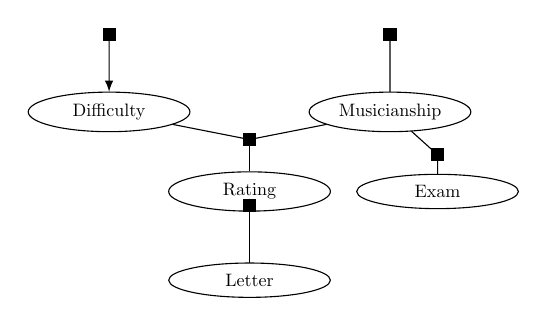
\begin{tikzpicture}[
  scale = 0.65, transform shape, 
  node distance=1cm and 0.5cm,
  mynode/.style={draw,ellipse,text width=2cm,align=center}
    ]

\node[mynode] (r) {Rating};
\node[draw, rectangle,above=of r,fill=black, yshift = -0.5cm] (fr) {};
\node[mynode,above left=of r] (d) {Difficulty};
\node[draw, rectangle,above=of d,fill=black] (fd) {};
\node[mynode,above right=of r] (m) {Musicianship};
\node[draw, rectangle,above=of m,fill=black] (fm) {};
\node[mynode,right=of r] (e) {Exam};
\node[draw, rectangle,above=of e,fill=black, yshift = -0.75cm] (fe) {};
\node[mynode,below=of r] (l) {Letter};
\node[draw, rectangle,above=of l,fill=black] (fl) {};
\path (fd) edge[-latex] (d)
(fm) edge (m)
(d) edge (fr)
(m) edge (fr)
(fr) edge (r)
(m) edge (fe)
(fe) edge (e)
(r) edge (fl)
(fl) edge (l);

\end{tikzpicture}

  \end{frame} 

\begin{frame}{Approximate Inference}

  For certain types of networks (singly connected) exact inference is
  reasonable but for the general case it can be shown to be NP-hard so
  it is not practical in many cases.

  Approximate inference methods are based on randomized sampling
  algorithms, also called {\bf Monte Carlo} algorithms that provide
  approximate answers whose accuracy depends on the number of samples
  generated and can deal with much larger networks. 
  
\end{frame}

\begin{frame}{A simple motivating example}
\begin{figure}[htb]
   \centering
   \includegraphics[width=6cm]{figures/snakes_ladders}
\end{figure}

\begin{itemize}
\item Draw N samples from sampling distribution
\item Compute an approximate posterior
\item Show that this approximate posterior converges to the true one
\end{itemize} 
\end{frame}

\begin{frame}{Direct Sampling}

  The basic idea is simple. Given a source of random numbers it is a
  simple matter to sample any discrete random variable. If the network
  has no evidence associated with it we can generate events by
  sampling each variable in turn in topological order. That way we
  always samples variables that are conditioned on values already
  assigned to the variable's parents.

  The outcome of the the process is an event i.e an assignment of
  values to each random variable. The answers are computed by counting
  the actual samples generated. For example if we generate $1000$
  samples from the musician network, and $712$ of them have {\it Exam =
    high} then the estimated probability of $\hat P(Exam = high)$ is
  $0.711$.
\end{frame}

\begin{frame}{Direct Sampling Example}
 \begin{itemize}
 \item Sample from $P(Difficulty) = <0.6,0.4>$; suppose it returns {\it high}
 \item Sample from $P(Musicianship) = <0.7,0.3>$; suppose it returns {\it weak}
   \item Sample from $P(Rating|Difficulty = high, Musicianship=weak) = <0.9, 0.08, 0.02>$; suppose it returns {\it **} 
   \item Sample from $P(Exam|Musicianship=weak)=<0.95,0.05>$; suppose it return {\it Low}
     \item Sample from $P(Letter|Rating=**)=<0.4, 0.6>$; suppose it return {\it Strong} 
   \end{itemize} 
 The randomly generated event will be: $[Difficulty=high, Musicianship=weak, Rating=**, Exam = low, Letter = strong]$. Repeat to generate more samples. 
\end{frame} 
  

\begin{frame}{Incorporating evidence - Rejection sampling}


  If we have some evidence we can still perform direct sampling and
  count the samples that are consistent with the
  evidence. Alternatively we can simply reject all samples that do not
  match the evidence and obtain the conditional estimate $\hat
  P(X=x|e)$ by counting how ofter $X=x$ occurs in the remaining
  samples. This is called {\bf rejection sampling}. However if the
  events for which the evidence is true are rare then we will have to
  generate a lot of samples to get enough to compute this estimate.
\end{frame} 


\begin{frame}{Likelihood weighting}
  
  {\bf Likelihood weighting} avoids this inefficiency of {\bf
    rejection sampling} by generating only events that are consistent
  with the evidence. When this is done not all generated events are
  equal. Before tallying the counts in the distribution for the query
  variable, each event is weighted by the {\it likelihood} that the
  events accords to the evidence.
  \end{frame} 

\begin{frame}{Markov Chain Monte Carlo (MCMC)}

  Unlike sampling algorithms that generate each event from scratch,
  MCMC generates each event by making a random change to the preceding
  event. It is useful to think of the network as being in a particular
  {\it state} specifying the value for each variable. The next state
  is generated by randomly sampling a value for one of the
  non-evidence variables $X_i$, conditioned on the current values of
  the variables in the Markov Blanket of $X_i$. MCMC wanders randomly
  around the state space, flipping one variable at a time {\it Gibbs
    sampling}, but keeping the evidence variables fixed. Many more
  variants exists but the basic principle of wandering in the state
  space is the same.

  Note: The Markov Blanket of a variable $X_i$ consists of its
  parents, children, and its children's other parents.
  
  \end{frame} 


\begin{frame}{Hybrid Bayesian Networks}

  Many real-world problems involve continuous quantities. A network
  with both discrete and continuous variables is called a {\bf Hybrid
    Bayesian Network}. To specify a hybrid network, we need to specify
  two kinds of distributions: conditional distributions for continuous
  variables given discrete or continuous parents, and conditional
  distributions for discrete variables given continous
  parents. Various techniques that are beyond the scope of this
  tutorial can be used to integrate continuous variables. In some
  cases that we will examine the structure is such that it is obvious
  how to combine the continuous and discrete variables for example in
  Hidden Markov Models.

  \end{frame} 


\begin{frame}{Dynamic Bayesian Networks}

  When we model phenomena over time we can view them as a sequence of
  snapshots.  Each snapshot describes the state of the world at a
  particular time described by random variables some of which are
  observable $E_t = e_t$ and some of which are not $X_t$.

  The {\bf Markov assumption} is that for all $t$:
  \[
  P(X_t | X_{0:t-1}) = (X_t | X_{t-1})
  \]
  and
  \[
  P(E_t | X_{0:t}, E_{0:t-1}) = P(E_t|X_t)
  \]
\end{frame}


\begin{frame}{Inference tasks in temporal models I} 

  \begin{itemize}
    \item {\bf Filtering:} we want to compute the posterior
      distribution over the current state, given all evidence to
      date. $P(X_t | e_{1:t})$. An almost identical calculation
      provides the likelihood of the evidence sequence $P(e_{1:T})$.
    \item {\bf Prediction:} we want to computer the posterior
      distribution over the future state, given all evidence to
      date. $P(X_{t+k} | e_{1:t})$ for some $k>0$.
    \item {\bf Smoothing or hindsight:} computing the posterior distribution over a past state, given all evidence up to the present: $P(X_K | e_{1:t})$ for some $k < t$. It provides a better estimate of the state than what was available at the time, because it incorporates more evidence.


    \end{itemize} 
\end{frame}

\begin{frame}{Inference tasks in temporal models II}
\begin{itemize} 
\item{\bf Most likely explanation:}

Given a sequence of observations, we might wish to find the sequence
of states that is most likely to have generated these
observations. That is we wish to compute:
$\argmax_{x_{1:t}}P(x_{1:t}|e_{1:t})$. This is the typical inference
task in Speech Recognition using Hidden Markov Models.

\end{itemize}

\end{frame}


\begin{frame}{Learning the transition and sensor models}

In addition to these tasks, we need methods for learning the
transition and sensor models from observations. The basic idea is that
inference provides an estimate of what transitions actually occurred
and what states generated the observations. These estimates can then be used
to update the models and the process can be repeated. This is an instance of the
{\bf expectation-maximization (EM)} algorithm. 

\end{frame} 

\begin{frame}{Sketch of filtering and prediction (Forward)}

  We perform {\bf recursive estimation}. First the current state
  distribution is projected forward from $t$ to $t+1$. Then it is
  updated using the new evidence $e_{t+1}$. We will not cover the
  details but it can be done by recursive application of Bayes rule
  and the Markove property of evidence and the sum/product rules.
  
  We can think of the filtered estimate $P(X_t | e_{1:t})$ as a
  ``message'' that is propagated forward alogn the sequence, modified
  by each transition, and updated by each new observation.
  
\end{frame}


\begin{frame}{Sketch of smoothing (Backward)}

  There are two parts to computing the distribution over past states
  given evidence up to the present. The first is the evidence up to
  $k$, and then the evidence from $k+1$ to $t$. The forward message
  can be computed as by filtering from $1$ to $k$. Using conditional
  independence and the sum and product rules we can form a backward
  message that runs backwards from $t$.

  It is possible to combine both steps in one pass to smooth the
  entire sequence. This is, not surprisingly, called the Foward-Backward
  algorithm. 
\end{frame}


\begin{frame}{Finding the most likely sequence}

View each sequence of states as a path through a graph whose nodes are
the possible states at each time step. The task is to find the most
likely path through this graph, where the likelihood of any path is
the product of the transition probabilities along the path and the
probabilities of the given observations at each state. Because of the
Markov property there is a recursive relationshtip between the most
likely paths to each state $x_{t+1}$ and most likely paths to each
state $x_t$. By running forward along the sequence, and computing $m$
messages at each time step we will have the probaiblity for the most
likely sequence reaching each of the final states. Then we simply
select the most likely one. This is called the {\bf Vitterbi
  algorithm}. 
  
  \end{frame} 

\begin{frame}{Connection to belief propagation} 

  The forward–backward algorithm in hidden Markov models (HMMs), and
  the Kalman smoothing algorithm in SSMs are both instances of belief
  propagation / factor graph propagation
  \end{frame} 


\begin{frame}{Linear-chain data}

  In music it is common to have structured data that form a linear
  chain over time. Examples include music instrumentation prediction
  and chord recognition.

  \includegraphics[width=10cm]{figures/linear_chain}  

\end{frame}


\begin{frame}{Notation for Linear Chain Data}
  \begin{itemize}
  \item {\bf x} is a sequence of observations
  \item {\bf y}  is the corresponding sequence of labels
  \item {\bf D} is a training set of such N (i.i.d) such
    sequences $\bf D = {{\bf x^{(1)},y^{(1)}}, \dots, {\bf x^{(N)},y^{(N)}}}$. 
\end{itemize} 
\end{frame}

\begin{frame}{Feature Functions}

  \begin{definition}{}
    A {\bf feature function} is a real-valued function of both the
    input sequence (observations) and the output space (target
    labels). It can be used to compute characteristics of the
    observations and associated constrains.
  \end{definition}

  Example:
  \[
  f_j(o_i, y_i) = \begin{cases}
    1 \;\;\; if \;\;\; o_i = C, o_{i+1} = E \;\;\; and \;\;\; y_i = Cmaj \\ 
    0 \;\;\; otherwise  \\ 
    \end{cases} 
  \]
  
  \end{frame} 

\begin{frame}{Conditional Random Fields}

\begin{definition}{CRF model definition}
\begin{eqnarray*} 
  p({\bf y} | {\pmb x; \pmb \theta}) =& \frac{1}{Z({\pmb x, \pmb \theta})}   
\exp  \sum_{j=1}^{D}{\theta_j F_j({\pmb x,\pmb y})} \\
=& \frac{1}{Z({\pmb x, \pmb \theta})} \Psi ({\pmb x,\pmb y, \pmb \theta}) \\
\end{eqnarray*}
\end{definition}

${Z({\pmb x, \pmb \theta})}$ is called a {\bf partition function},
and $\Psi ({\pmb x,\pmb y, \pmb \theta})$ is called a {\bf ponential function}.
Feature functions can depend on the whole sequence of observation and labels. 
\end{frame}

\begin{frame}{Feature functions as constraints}

  We can express varioust types of constraints through feature
  functions.  For example for a linear-chain CRF each feature function
  depends on the whole sequence of observations but only on the {\bf
    current} and {\bf previous} labels. One can define {\bf
    observation feature functions} and {\bf transition feature
    functions}.

  It can be shown that HMMs are a special case of linear chair CRFs
  with appropriately defined feature functions. 
\end{frame} 

\begin{frame}{Differences of CRFs with HMMs}

  CRFs have a number of advantages over HMMs based on the following differences :
\begin{itemize}
\item CRFs are discriminative models
\item CRFs are undirected models 
\end{itemize}

   \includegraphics[width=10cm]{figures/crf_hmm}

   As is the case with any probabilistic model we can perform
   inference given a model and we need to learn the parameters of the
   model given a training set.
   
\end{frame}

\begin{frame}{Hands-on Bayesian Network}

  Jupyter notebook for exploring Bayesian Networks and inference. 
  \end{frame} 



\section{Markov Logic Networks (with Helene Papadopoulos)} 
\begin{frame}
\frametitle{Estimation of Content Information from Audio Signals of Music: State-of-the-art}

\textcolor{red}{What are the limitation of existing approaches for estimating content information from music signals?}
\bigskip

\begin{itemize}

\item Most existing computational models tend to focus on a single music attribute (chord, beat, structure, etc.).
\smallskip

\textcolor{red}{$\rightarrow$} It is contrary to the human understanding and perception of music that processes holistically the global musical context.% \textcolor{violet}{[3]}. 
\bigskip

\end{itemize} 
\end{frame}

\begin{frame}{What is needed} 

\textcolor{red}{What are the limitation of existing approaches for estimating content information from music signals?}
\bigskip
\begin{itemize} 
\item Dealing with real audio recordings requires the ability to handle both:
\smallskip

\begin{itemize}
	\item Rich probabilistic and 
	\item Complex relational structure at multiple levels of representation. 
\end{itemize}
\smallskip
\textcolor{red}{$\rightarrow$} Existing approaches for musical retrieval tasks fail to capture both of these aspects.

\end{itemize}
\end{frame}


\begin{frame}
\frametitle{Probabilistic Graphical Models}

\textcolor{red}{Probabilistic graphical models are popular in MIR}
\bigskip 

\begin{itemize}

\item \textcolor{blue}{Hidden Markov models (HMM)} are successful in modeling tasks where objects can be represented as sequential phenomena: 
\begin{itemize}
	\item Chord estimation \textcolor{violet}{[Sheh \& Ellis 2003]}, beat tracking \textcolor{violet}{[Klapuri \textit{et al.}  2006]} etc.
	\item \textcolor{blue}{Limitation}: hard to express dependencies in the data. 
\medskip

\item Other formalisms allow more complex dependencies:
  \end{itemize}
\begin{itemize}
\item Conditional random fields \textcolor{violet}{[Burgoyne \textit{et al.} 2007]}, N-grams \textcolor{violet}{[Scholz \textit{et al.} 2008]} or tree structures \textcolor{violet}{[Paiement \textit{et al.} 2005]}.
  
\end{itemize}
\end{itemize} 
\end{frame} 

\begin{frame}{Limitations of probabilistic graphical models}
\begin{itemize}   
\item Although probabilistic models can handle the inherent
  uncertainty of audio, most of them fail to capture important aspects
  of \textcolor{blue}{higher-level musical relational structure and
    context}.
\medskip
\item This aspect has been more specifically explored within the framework of \textcolor{blue}{Logic}.
\end{itemize}
\end{frame}

%%%%%%%%%%%%%%%%%%%%%%%%%%%%%%%%%%%%%%%%%%%%%%%%%%%%%%%%%%%%%%%%
\begin{frame}
\frametitle{Logic Frameworks and expressiveness}
\begin{itemize}
\item Modelling music rules is \textcolor{blue}{compact and human-readable}:
\begin{itemize}
	\item Intuitive description of music.
	\item Knowledge (e.g. music theory) can reflected in rules:  \textcolor{blue}{\textit{``CM chord $\wedge$ first degree $\Rightarrow$ CM key''}}% \textcolor{violet}{[9]}. 
\end{itemize}

\item \textcolor{blue}{Inductive Logic Programming (ILP)} \textcolor{violet}{[Muggleton 1991]} that combines \textcolor{blue}{logic programming} with \textcolor{blue}{machine learning} has been used to model and learn music rules:
\begin{itemize}
	\item Harmony characterization \textcolor{violet}{[Anglade \& Dixon 2008]}.
	\item Expressive music performance \textcolor{violet}{[Ramirez \textit{et al.} 2007]}. 
\end{itemize}

\item \textcolor{blue}{Limitations}: 
\begin{itemize}
	\item Logic-based approaches have focused on symbolic representations (e.g. MIDI).
	\item Applying these approaches to audio generally requires a transcription step.
\end{itemize}

\end{itemize}
\end{frame}

%%%%%%%%%%%%%%%%%%%%%%%%%%%%%%%%%%%%%%%%%%%%%%%%%%%%%%%%%%%%%%%%
\begin{frame}
\frametitle{Markov Logic for the Analysis of Music Signals}

\textcolor{red}{Markov Logic Networks} (MLNs)
\textcolor{violet}{[Richardson \& Domingos 2006]} as an expressive
formalism to estimate music content information from audio signals.
%\vspace{-0.7cm} 
\begin{figure}[htb]
   \centering
   \includegraphics[width=10cm]{figures/Figure_MLN-eps-converted-to}
\end{figure}

\end{frame}

%%%%%%%%%%%%%%%%%%%%%%%%%%%%%%%%%%%%%%%%%%%%%%%%%%%%%%%%%%%%%%%%


\begin{frame}
\frametitle{Markov Logic for Modeling Chord Progressions}

\textcolor{red}{Problem:} Estimate the harmonic progression of an audio music signal 
at the analysis-frame level, taking into account a more global semantic level. Audio signals contain music notes that correspond to a chord sequence over time. 
\vspace{-0.5cm}
%\vspace{-1cm}
\begin{columns}[c] 
\begin{column}{0.55\textwidth} 
\begin{itemize}
\item What are these notes? (\textcolor{blue}{physical complexity})
\item  Which chords do they represent? (\textcolor{blue}{semantic complexity})
\item  Segmentation: chord labels related to the global semantic structure (\textcolor{blue}{complex relational structure})

%\item $\rightarrow$ Chord labels $\&$ segmentation

\end{itemize}
\end{column} 

\begin{column}{0.45\textwidth} 
%\vspace{-0.5cm}
\begin{figure}[htb]
   \centering
   \includegraphics[height=3cm]{figures/chord_extraction_BurSau2005-eps-converted-to}
   \caption{Adapted from \textcolor{violet}{[Burgoyne and Saul 2005]}.}
\end{figure}
\end{column}
\end{columns}
\medskip 

% We consider a chord lexicon of 24 major and minor triads (CM,.., BM,.., Bm) (\textcolor{blue}{mid-level representation}).


\end{frame}
%%%%%%%%%%%%%%%%%%%%%%%%%%%%%%%%%%%%%%%%%%%%%%%%%%%%%%%%%%%%%%%%


\begin{frame}
\frametitle{Structurally consistentモ mid-level \\ representation of music}

\textcolor{red}{Considered  problem:} Estimating the harmonic progression of an audio music signal considering several time-scales of representation.
%
\bigskip 


\begin{itemize}
\item Music pieces are \textcolor{blue}{structured at several time scales}, from musical phrases to longer sections that generally have \textcolor{blue}{multiple occurrences}. 

\item Here, \textcolor{blue}{popular music}: pieces can be segmented into specific repetitive segments with labels such as \textit{chorus}, \textit{verse}, or \textit{refrain}. 
\medskip

\item Segments are considered as similar here if they represent the \textcolor{blue}{same musical content}. 
\medskip

\item In particular, two same segment types are likely to have \textcolor{blue}{similar harmonic structures}. 
\medskip

\end{itemize}

\end{frame}


%%%%%%%%%%%%%%%%%%%%%%%%%%%%%%%%%%%%%%%%%%%%%%%%%%%%%%%%%%%%%%%%
\begin{frame}
\frametitle{Structurally consistentモ mid-level representation I}

\textcolor{red}{Previous work}: music structure as a constraint:	
\begin{itemize}	
	\item \textcolor{violet}{[Dannenberg 2005]}: constraint to a beat tracking program.	
	\item \textcolor{violet}{[Mauch \textit{et al.} 2009]}: context information for chord estimation.	
\end{itemize}
\bigskip
%\item \textcolor{blue}{Limitation}: .  An instance of \textcolor{blue}{blurred} segment features (e.g. noise or percussive sounds) will automatically affect all same segments.

%\item \textcolor{blue}{Proposed approach}: Using prior structural information to enhance chord estimation in a \textcolor{blue}{more elegant and flexible way} within the framework of \textcolor{blue}{Markov Logic Networks}.
%\begin{itemize}
%	\item We only \textcolor{blue}{favor} same chord progressions for all instances of the same segment type (no hard constraint). Take into account \textcolor{blue}{variations} between several occurrences
%	\item Potential of  incorporating more context information and discovering new predicates.
%\end{itemize}


	%\item Extract features from the signal, and segments corresponding to a given type of section are replaced by the average of the chromagram over all the instance of the same segment type over the whole song, so that similar structural segments are labelled with the exact same chord progression. 
%\end{itemize}
	
\begin{columns}[c] 

\begin{column}{0.5\textwidth} 
\vspace{-0.4cm}
\begin{figure}[htb]
   \centering
   \includegraphics[width =\textwidth]{figures/Meth_MD.eps}%0.4\textwidth
\end{figure}
\end{column} 

\begin{column}{0.5\textwidth} 
%\vspace{-0.2cm}
\textcolor{blue}{Limitations}:
\begin{itemize}	
	%\item hypothesis that the \textcolor{blue}{music content} is \textcolor{blue}{exactly} the same in all sections of the same type.
	\item Repeated segments often present \textcolor{blue}{variations} between several occurrences. 
	\item An instance of \textcolor{blue}{blurred} segment features (e.g. noise or percussive sounds) will automatically affect all same segments.
\end{itemize}
\end{column} 

\end{columns} 

%\begin{itemize}
%\item \textcolor{red}{Proposed approach}: Using \textcolor{blue}{prior} structural information to enhance chord estimation in a \textcolor{blue}{more elegant and flexible way} within the framework of \textcolor{blue}{MLNs}.
%\begin{itemize}
%	\item No hard constraint:  we only \textcolor{blue}{favor} same chord progressions for all instances of the same segment type.
%	\item Potential of  incorporating more context information and discovering new predicates.
%\end{itemize}
%\end{itemize}


\end{frame}

%%%%%%%%%%%%%%%%%%%%%%%%%%%%%%%%%%%%%%%%%%%%%%%%%%%%%%%%%%%%%%%%
\begin{frame}
\frametitle{Proposed Approach}

Using \textcolor{blue}{prior structural information} to enhance chord estimation in a \textcolor{blue}{more elegant and flexible way} using \textcolor{blue}{Markov Logic Networks}.
\begin{itemize}
	\item The model is not constrained to have the exact same chord progression in all sections of the same type (\textcolor{blue}{no hard constraint}) .
	\item But we only \textcolor{blue}{favor} same chord progressions for all instances of the same segment type.
	\item Potential of  incorporating more context information and discovering new predicates.
\end{itemize}

\textcolor{red}{Hypothesis}
\begin{itemize}
	\item Song segmentation in beats and structure is given 
	\item Similar segment instances have the same length in beats.
\end{itemize}



\end{frame}

%%%%%%%%%%%%%%%%%%%%%%%%%%%%%%%%%%%%%%%%%%%%%%%%%%%%%%%%%%%%%%%%

\begin{frame}
\frametitle{Markov Logic Networks (MLN): short overview}

A \textcolor{red}{Markov Logic Network} is a set of \textcolor{blue}{weighted first-order logic formulas} that can be seen as a template for the construction of a probabilistic graphical model.
\medskip

A \textcolor{red}{first-order knowledge base} (KB) is a set of formulas in first-order logic that can be seen as a set of \textcolor{blue}{hard constraints} on the set of possible worlds.

\begin{small}
\begin{itemize}
\item First-order KB: if a world violates even one formula, it has zero probability. 
\item In \textit{real world schemes}, logic formulas are \textit{generally} true, but \textit{not always}. 
\end{itemize}
\end{small}
\medskip
\end{frame}

\begin{frame}
\frametitle{MLN overview II}
\textcolor{red}{Basic idea in Markov logic:} to soften these constraints to handle uncertainty. The weights reflect how strong a constraint is.
\medskip

\begin{columns}[c] 
\begin{column}{0.65\textwidth} 

\vspace{-0.3cm}
\begin{figure}[htb]
   \centering
   \includegraphics[height=2cm]{figures/exemple_KB.eps}
\end{figure}

\vspace{-0.6cm}
\begin{figure}[htb]
   \centering
   \includegraphics[height=2cm]{figures/MLN_KB.eps}
\end{figure}

\end{column} 

\begin{column}{0.35\textwidth} 
\vspace{-0.2cm}

\textit{Example of a first-order KB and corresponding weights in the MLN.}

\vspace{0.8cm}

\textit{Ground Markov network obtained by applying the formulas to the \textcolor{red}{constants} CM and GM chord.}

\end{column} 
\end{columns} 
\end{frame}



%%%%%%%%%%%%%%%%%%%%%%%%%%%%%%%%%%%%%%%%%%%%%%%%%%%%%%%%%%%%%%%

\begin{frame}
\frametitle{Modeling harmonic content of audio signals}

\bigskip

\textcolor{blue}{Chroma representation:} Mapping of spectrum
to a 12-dimensional vector representing the intensity of the 12
semitone pitch classes.
\medskip


\vspace{-0.5cm}
\begin{figure}[htb]
   \centering
   \includegraphics[width = 10cm]{figures/chromagram.eps}
\end{figure}

\textcolor{blue}{Beat-synchronous chroma feature:} observation features related to the meter (beat tracking algorithm \textcolor{violet}{[Peeters 2007]}).

\end{frame}

%%%%%%%%%%%%%%%%%%%%%%%%%%%%%%%%%%%%%%%%%%%%%%%%%%%%%%%%%%%%%%%



\begin{frame}
\frametitle{HMM Chord Detection}

\textcolor{red}{Classical approach}: Hidden Markov Model (HMMs) have been widely used to model the chord progression of an audio file \textcolor{violet}{[Sheh $\&$ Ellis 2003], [Bello $\&$ Pickens 2005], [Lee 2006]} etc.
%\item One of the main reasons: The transitions between chords result from musical rules that can be modeled in a state transition matrix.
\vspace{-0.4cm} 

\vspace{-0.4cm}
\hspace{-0.4cm}
 \begin{figure}[htb]
   \centering 
   \includegraphics[width = 11.5cm]{figures/chord_HMM.eps}
\end{figure}
\end{frame}

\begin{frame}
\frametitle{HMM Chord Detection} 

\textcolor{red}{Classical approach}: Hidden Markov Model (HMMs): 
%\item One of the main reasons: The transitions between chords result from musical rules that can be modeled in a state transition matrix.

\begin{columns}[c] 

\begin{column}{0.6\textwidth} 
\vspace{-0.4cm}
\begin{figure}[htb]
   \centering
   \includegraphics[height=3cm]{figures/HMM.eps}
\end{figure}
\begin{itemize}	
\item The observation (chroma) tells us something about the state.
\item The transitions between states follows a transition probability distribution
\end{itemize}

\end{column} 


\begin{column}{0.4\textwidth} 
\vspace{-0.5cm}
\begin{figure}[htb]
   \centering
   \includegraphics[height=3cm]{figures/best_path.eps}
\end{figure}
The chord progression over time is estimated in a \textcolor{blue}{maximum likelihood sense} using the \textcolor{blue}{Viterbi decoding algorithm}.
\end{column} 

\end{columns} 


\end{frame}

\begin{frame}
\frametitle{From HMMs to MLNs}

The chord progression can be \textcolor{blue}{equivalently} modeled in
the MLN framework using \textcolor{blue}{three generic weighted
  logical formulas} that reflect the constraints defining the HMM.
\medskip 

\begin{columns}[c] 

\begin{column}{0.62\textwidth} 
\vspace{-2.0cm}
\begin{figure}[htb]
   \centering
   \includegraphics[height=5cm]{figures/MLN_chord_couleur.eps}\vspace{-0.2cm}
%   \caption{\small \textit{Structure of the domain: MLN for chord progression description (same weights than the HMM parameters).}}
\end{figure}
\end{column} 


\begin{column}{0.38\textwidth} 
Structural information is incorporated using the time \textcolor{blue}{temporal predicate $Succ(t_{1},t_{2})$} that indicates the position of successive frames.

\vspace{-0.5cm}
\begin{figure}[htb]
   \centering
   \includegraphics[height=1.7cm]{figures/Evidence_MLN_chord_couleur.eps}%\vspace{-0.cm}
%   \caption{\small \textit{Evidence for chord progression description.}}
\end{figure}

\end{column} 

\end{columns} 




\end{frame}

%% %%%%%%%%%%%%%%%%%%%%%%%%%%%%%%%%%%%%%%%%%%%%%%%%%%%%%%%%%%%%%%%



\begin{frame}
\frametitle{Chord Progression: Global Semantic Structure}

\textcolor{red}{Flexibility of MLN: \textit{Prior global structural information}}
\medskip 

%\begin{itemize}
%\item The time predicate \textcolor{blue}{$SuccStr$} allows considering wider temporal windows, as opposed to consecutive frames via the \textcolor{blue}{$Succ$} predicate.

Formulas added to express the constraint that \textcolor{blue}{\textit{two same segment types are likely to have a similar chord progression}}.
%\end{itemize}
\medskip 

\begin{columns}[c] 

\begin{column}{0.6\textwidth} 


\vspace{-1.0cm}
\begin{figure}[htb]
   \centering
   \includegraphics[height=5cm]{figures/MLN_chord_struct_couleur.eps}
   %\caption{\small MLN for joint chord and structure description.}
\end{figure}
\end{column} 

\begin{column}{0.4\textwidth} 

\vspace{-0.2cm}
The predicate \textcolor{blue}{$SuccStr$} allows considering wider windows, as opposed to consecutive frames via the \textcolor{blue}{$Succ$} predicate.
%For each pair of same segment type, the position of matching beat-synchronous frames (likely to be the same chord type) is given as evidence:

\vspace{-0.3cm}
\begin{figure}[htb]
   \centering
   \includegraphics[height=2.8cm]{figures/Evidence_MLN_chord_struct_couleur.eps}
   %\caption{\small Evidence for chord and structure description.}
\end{figure}

\end{column} 

\end{columns} 

\end{frame}


%% %%%%%%%%%%%%%%%%%%%%%%%%%%%%%%%%%%%%%%%%%%%%%%%%%%%%%%%%%%%%%%%



\begin{frame}
\frametitle{Inference}

\textcolor{red}{How to  estimate the chord progression?}
\medskip 

\begin{itemize}
\item \textcolor{blue}{Query:} Find the chord progression \textcolor{blue}{Given:} 

\item The \textcolor{blue}{structure of the domain:} represented by a set of logical formulas (rules) $F_{i}$, with attached weight $w_{i}$.

\item A set of \textcolor{blue}{evidence} literals (chroma observations, position of consecutive frames and same segment types).
\end{itemize}
\medskip 

%\textcolor{red}{Query} : the chord progression



\textcolor{blue}{Maximum A Posteriori} (MAP) inference, finds the most probable state given the evidence.
\medskip 

%\textcolor{blue}{Maximum A Posteriori} (MAP) inference, finds the most probable state of the world $y$ given some evidence $x$:
%\noindent
%\begin{small}
%\abovedisplayskip=2pt
%\belowdisplayskip=2pt
%\begin{eqnarray}
%\underset{y}{\operatorname{argmax}}\ P(y|x) = &\underset{y}{\operatorname{argmax}}\frac{1}{Z} exp(\sum_{i}w_{i}n_{i}(x,y)) \nonumber
%%&= \underset{y}{\operatorname{argmax}}\sum_{i}w_{i}n_{i}(x)
%\vspace{-0.2cm}
%\end{eqnarray}
%\end{small}

For inference, we used the exact solver toulbar2 \textcolor{blue}{branch \& bound} MPE inference \textcolor{violet}{[Allouche \textit{et al.} 2010]} with the \textcolor{blue}{ProbCog} toolbox \textcolor{violet}{[Jain 2011]}.

\end{frame}



%% %%%%%%%%%%%%%%%%%%%%%%%%%%%%%%%%%%%%%%%%%%%%%%%%%%%%%%%%%%%%%%%



\begin{frame}
\frametitle{Results}


\vspace{-0.4cm}
\begin{columns}[c] 

\begin{column}{0.5\textwidth} 
\begin{itemize}

\item \textcolor{red}{Test-set}: 143 hand-labeled Beatles songs
\textcolor{red}{$\rightarrow$} Removing songs for which the structure was ambiguous.

\item \textcolor{red}{Evaluation measure}: chord label accuracy.%  \textcolor{red}{$\rightarrow$} mean and standard deviation of correctly identified chords per song. 
\end{itemize}
\end{column} 


\begin{column}{0.5\textwidth} 
\begin{figure}[htb]
   \centering
   \includegraphics[height=1.5cm]{figures/result_MLN.eps}\vspace{-0.3cm}
   \caption {\footnotesize \textit{MLN\_struct: MLN incorporating prior structural information, MLN\_chord: baseline HMM, [36]: chromagram averaged over same segment types as in \textcolor{violet}{[Mauch \textit{et al.} 2009]}.}}
   %\caption {\textit{MLN\_struct}: MLN incorporating prior structural information, \textit{MLN\_chord}: baseline HMM, [36]: chromagram average as in \textcolor{violet}{[Mauch \textit{et al.} 2009]}.}
\end{figure}

\end{column} 
\end{columns} 
\medskip
\end{frame} 

\begin{frame} 
\frametitle{Results}
\vspace{-0.6cm}
\begin{figure}[htb]
   \centering
   \includegraphics[height=2cm]{figures/OneAfter909_font16_annote_petit_slides_rouge.eps}
   \vspace{-0.4cm}
   \caption {\footnotesize \textit{Chord estimation results for an excerpt of the song One After 909}}.
\end{figure}

\vspace{-0.7cm}
Global semantic information can be \textcolor{blue}{concisely and elegantly combined} with information at the beat-synchronous time scale: 

\textcolor{red}{$\rightarrow$} Chord estimation results are significantly improved, and more consistent with the global structure (\textcolor{red}{see the grey dashed rectangles}).

\textcolor{red}{$\rightarrow$} Variations between segments are taken into account (\textcolor{red}{see the black dashed rectangles}).

\end{frame}


\begin{frame} 
\frametitle{Results of Key and Chord Estimation \\ using Markov Logic Networks}
Improving chord estimation using provided key information. Joint
estimation provides key estimation for free.

\begin{figure}[htb]
   \centering
   \includegraphics[width=10cm]{figures/mln_key.png}
\end{figure}

\begin{figure}[htb]
   \centering
   \includegraphics[width=10cm]{figures/mln_key_2.png}
\end{figure}



\end{frame} 


\begin{frame}
\frametitle{Music Content Estimation using Markov Logic}


\begin{itemize}
\item Markov logic: a formalism that enables \textcolor{blue}{intuitive, effective, flexible and expressive} reasoning about complex relational structure and uncertainty of music data. 
\medskip

\item New step towards a unified multi-level description of audio at various time-scales, in which information specific to various semantic levels (analysis frame, phrase and global structure) interact.


\item Future work: extend this approach to a fully automatic one (incorporating estimated beats and structure location).

\end{itemize}
\end{frame} 


\begin{frame}{Future work}

Major objectives: 

\begin{itemize}
	\item Automatically discover and model new structural rules with learning algorithms.
	\item Take advantage of the flexibility of the MLN to combine training iformation with background music knowledge.
\end{itemize}
\end{frame}

\begin{frame}
\frametitle{Open questions - future work}

\begin{itemize}
\item{ Think in parallel about a ``good signal representation'' and the ``models for information extraction''.} 
\medskip 
\item Fully integrate in the model chord and beat estimation in an interactive fashion (e.g. update the chromagram with the other parameters during MCMC inference in order to possibly improve the chord estimation).
\medskip
\item Incorporate more music knowledge / mid-level representations of audio (structure, instrumentation etc.) to inform signal representation. 
\medskip 
\item Build models that take into account complex relational structures and uncertainty of real audio. 
\medskip
\item Towards a multi-scale signal analysis at multiple semantic levels in a complex acoustical environment.
\end{itemize}
\end{frame}


\begin{frame}{More open questions}
\begin{itemize} 
\item Improve the priors (e.g. by using a time segmentation, a larger chord lexicon, using onsets combined with beat positions etc.). 
\item Extend the model so that dependencies \textit{between} layers are taken into account

\item Future work: extend this approach to a fully automatic one (incorporating estimated beats and structure location). 
\medskip

\item Major objectives: 
\end{itemize}
\begin{itemize}
	\item Automatically discover and model new structural rules with learning algorithms.
	\item Take advantage of the flexibility of the MLN to combine training information with background music knowledge.
\end{itemize}
\end{frame}


\begin{frame}
\frametitle{Markov Logic Networks in Music}

\begin{center}
Thank you for your attention!
\end{center}
\bigskip

%\justifyit
\begin{small}

\begin{center}
\rmfamily\textsc{Related publications}\normalfont
\end{center}

H. Papadopoulos and G. Tzanetakis. \textcolor{blue}{Models for Music Analysis
  from a Markov Logic Perspective}, \textit{IEEE/ACM Transactions on Audio, Speech and Language Processing}, 25(1), 19-34, 2016. 

H. Papadopoulos and G. Tzanetakis. \textcolor{blue}{Exploiting Structural Relationships in Audio Music Signals Using Markov Logic Networks}, \textit{Proceedings of ICASSP}, 2013.
\medskip

H. Papadopoulos and G. Tzanetakis. \textcolor{blue}{Modeling Chord and Key Structure with Markov Logic}, \textit{Proceedings of ISMIR}, 2012.
\medskip

\end{small}

\end{frame}

\section{Conclusion} 

\begin{frame}{Summary}

  Probabilistic modeling allows us to formulate and solve many
  interesting problems in music analysis and signal processing in
  general. It allows us to express our assumptions and associated
  uncertainties and learn from data. By using inference we can solve a
  variety of interesting problesm based on the same underlying model.
  It is easy to get lost in the details of individual algorithms and
  models but once you start understanding the basic concepts it
  becomes easier to make sense of the literature. I hope that this
  tutorial helped you formulate this big picture view of model-based
  probabilistic machine learning.
  
  \end{frame} 

\setbeamercolor{bibliography item}{fg=black}
\setbeamercolor*{bibliography entry title}{parent=palette primary}

\bibliographystyle{amsalpha}
\bibliography{dhsi_2014} 




\end{document}











